% Options for packages loaded elsewhere
\PassOptionsToPackage{unicode}{hyperref}
\PassOptionsToPackage{hyphens}{url}
\PassOptionsToPackage{dvipsnames,svgnames,x11names}{xcolor}
%
\documentclass[
  letterpaper,
  DIV=11,
  numbers=noendperiod]{scrartcl}

\usepackage{amsmath,amssymb}
\usepackage{iftex}
\ifPDFTeX
  \usepackage[T1]{fontenc}
  \usepackage[utf8]{inputenc}
  \usepackage{textcomp} % provide euro and other symbols
\else % if luatex or xetex
  \usepackage{unicode-math}
  \defaultfontfeatures{Scale=MatchLowercase}
  \defaultfontfeatures[\rmfamily]{Ligatures=TeX,Scale=1}
\fi
\usepackage{lmodern}
\ifPDFTeX\else  
    % xetex/luatex font selection
\fi
% Use upquote if available, for straight quotes in verbatim environments
\IfFileExists{upquote.sty}{\usepackage{upquote}}{}
\IfFileExists{microtype.sty}{% use microtype if available
  \usepackage[]{microtype}
  \UseMicrotypeSet[protrusion]{basicmath} % disable protrusion for tt fonts
}{}
\makeatletter
\@ifundefined{KOMAClassName}{% if non-KOMA class
  \IfFileExists{parskip.sty}{%
    \usepackage{parskip}
  }{% else
    \setlength{\parindent}{0pt}
    \setlength{\parskip}{6pt plus 2pt minus 1pt}}
}{% if KOMA class
  \KOMAoptions{parskip=half}}
\makeatother
\usepackage{xcolor}
\setlength{\emergencystretch}{3em} % prevent overfull lines
\setcounter{secnumdepth}{5}
% Make \paragraph and \subparagraph free-standing
\makeatletter
\ifx\paragraph\undefined\else
  \let\oldparagraph\paragraph
  \renewcommand{\paragraph}{
    \@ifstar
      \xxxParagraphStar
      \xxxParagraphNoStar
  }
  \newcommand{\xxxParagraphStar}[1]{\oldparagraph*{#1}\mbox{}}
  \newcommand{\xxxParagraphNoStar}[1]{\oldparagraph{#1}\mbox{}}
\fi
\ifx\subparagraph\undefined\else
  \let\oldsubparagraph\subparagraph
  \renewcommand{\subparagraph}{
    \@ifstar
      \xxxSubParagraphStar
      \xxxSubParagraphNoStar
  }
  \newcommand{\xxxSubParagraphStar}[1]{\oldsubparagraph*{#1}\mbox{}}
  \newcommand{\xxxSubParagraphNoStar}[1]{\oldsubparagraph{#1}\mbox{}}
\fi
\makeatother


\providecommand{\tightlist}{%
  \setlength{\itemsep}{0pt}\setlength{\parskip}{0pt}}\usepackage{longtable,booktabs,array}
\usepackage{calc} % for calculating minipage widths
% Correct order of tables after \paragraph or \subparagraph
\usepackage{etoolbox}
\makeatletter
\patchcmd\longtable{\par}{\if@noskipsec\mbox{}\fi\par}{}{}
\makeatother
% Allow footnotes in longtable head/foot
\IfFileExists{footnotehyper.sty}{\usepackage{footnotehyper}}{\usepackage{footnote}}
\makesavenoteenv{longtable}
\usepackage{graphicx}
\makeatletter
\newsavebox\pandoc@box
\newcommand*\pandocbounded[1]{% scales image to fit in text height/width
  \sbox\pandoc@box{#1}%
  \Gscale@div\@tempa{\textheight}{\dimexpr\ht\pandoc@box+\dp\pandoc@box\relax}%
  \Gscale@div\@tempb{\linewidth}{\wd\pandoc@box}%
  \ifdim\@tempb\p@<\@tempa\p@\let\@tempa\@tempb\fi% select the smaller of both
  \ifdim\@tempa\p@<\p@\scalebox{\@tempa}{\usebox\pandoc@box}%
  \else\usebox{\pandoc@box}%
  \fi%
}
% Set default figure placement to htbp
\def\fps@figure{htbp}
\makeatother
% definitions for citeproc citations
\NewDocumentCommand\citeproctext{}{}
\NewDocumentCommand\citeproc{mm}{%
  \begingroup\def\citeproctext{#2}\cite{#1}\endgroup}
\makeatletter
 % allow citations to break across lines
 \let\@cite@ofmt\@firstofone
 % avoid brackets around text for \cite:
 \def\@biblabel#1{}
 \def\@cite#1#2{{#1\if@tempswa , #2\fi}}
\makeatother
\newlength{\cslhangindent}
\setlength{\cslhangindent}{1.5em}
\newlength{\csllabelwidth}
\setlength{\csllabelwidth}{3em}
\newenvironment{CSLReferences}[2] % #1 hanging-indent, #2 entry-spacing
 {\begin{list}{}{%
  \setlength{\itemindent}{0pt}
  \setlength{\leftmargin}{0pt}
  \setlength{\parsep}{0pt}
  % turn on hanging indent if param 1 is 1
  \ifodd #1
   \setlength{\leftmargin}{\cslhangindent}
   \setlength{\itemindent}{-1\cslhangindent}
  \fi
  % set entry spacing
  \setlength{\itemsep}{#2\baselineskip}}}
 {\end{list}}
\usepackage{calc}
\newcommand{\CSLBlock}[1]{\hfill\break\parbox[t]{\linewidth}{\strut\ignorespaces#1\strut}}
\newcommand{\CSLLeftMargin}[1]{\parbox[t]{\csllabelwidth}{\strut#1\strut}}
\newcommand{\CSLRightInline}[1]{\parbox[t]{\linewidth - \csllabelwidth}{\strut#1\strut}}
\newcommand{\CSLIndent}[1]{\hspace{\cslhangindent}#1}

\usepackage{booktabs}
\usepackage{longtable}
\usepackage{array}
\usepackage{multirow}
\usepackage{wrapfig}
\usepackage{float}
\usepackage{colortbl}
\usepackage{pdflscape}
\usepackage{tabu}
\usepackage{threeparttable}
\usepackage{threeparttablex}
\usepackage[normalem]{ulem}
\usepackage{makecell}
\usepackage{xcolor}
\KOMAoption{captions}{tableheading}
\makeatletter
\@ifpackageloaded{caption}{}{\usepackage{caption}}
\AtBeginDocument{%
\ifdefined\contentsname
  \renewcommand*\contentsname{Table of contents}
\else
  \newcommand\contentsname{Table of contents}
\fi
\ifdefined\listfigurename
  \renewcommand*\listfigurename{List of Figures}
\else
  \newcommand\listfigurename{List of Figures}
\fi
\ifdefined\listtablename
  \renewcommand*\listtablename{List of Tables}
\else
  \newcommand\listtablename{List of Tables}
\fi
\ifdefined\figurename
  \renewcommand*\figurename{Figure}
\else
  \newcommand\figurename{Figure}
\fi
\ifdefined\tablename
  \renewcommand*\tablename{Table}
\else
  \newcommand\tablename{Table}
\fi
}
\@ifpackageloaded{float}{}{\usepackage{float}}
\floatstyle{ruled}
\@ifundefined{c@chapter}{\newfloat{codelisting}{h}{lop}}{\newfloat{codelisting}{h}{lop}[chapter]}
\floatname{codelisting}{Listing}
\newcommand*\listoflistings{\listof{codelisting}{List of Listings}}
\makeatother
\makeatletter
\makeatother
\makeatletter
\@ifpackageloaded{caption}{}{\usepackage{caption}}
\@ifpackageloaded{subcaption}{}{\usepackage{subcaption}}
\makeatother

\usepackage{bookmark}

\IfFileExists{xurl.sty}{\usepackage{xurl}}{} % add URL line breaks if available
\urlstyle{same} % disable monospaced font for URLs
\hypersetup{
  pdftitle={Introduction},
  pdfauthor={Magnus Johansson, PhD},
  pdfkeywords={Rasch, Psychometrics, Item fit, Cutoffs, Critical
values, Model fit},
  colorlinks=true,
  linkcolor={blue},
  filecolor={Maroon},
  citecolor={Blue},
  urlcolor={Blue},
  pdfcreator={LaTeX via pandoc}}


\title{Introduction}
\author{Magnus Johansson, PhD}
\date{2025-01-12}

\begin{document}
\maketitle
\begin{abstract}
Psychometrics in general have long relied on rule-of-thumb critical
values for various goodness of fit metrics. With more powerful personal
computers it is both feasible and desirable to use simulation methods to
determine appropriate critical cutoff values. This paper illustrates and
evaluates the use of an R package for Rasch psychometrics that has
implemented functions to simplify the process of determining simulation
based cutoff values. Through a series of simulation studies, a
comparison is made between the two methods of information-weighted
conditional item fit (``infit'') and item-restscore correlations using
Goodman and Kruskal's \(\gamma\). Results indicate the limitations of
small samples (n \textless{} 500) in correctly detecting item misfit due
to multidimensionality, especially when a larger proportion of items are
misfit. Item outfit shows very low performance in general. Conditional
infit with simulation-based cutoffs performs better than item-restscore
with sample sizes below 500. Both methods result in problematic rates of
false positives with large samples (n \textgreater= 1000). Large
datasets should be analyzed using nonparametric bootstrap of subsamples
with item-restscore to reduce the risk of type-1 errors. Finally, the
importance of an iterative analysis process is emphasized, since a
situation where several items show underfit will cause other items to
show overfit to the Rasch model. Underfit items should be removed one at
a time, and a re-analysis conducted for each step to avoid erroneously
eliminating items.
\end{abstract}


This paper presents a series of simulations conducted to evaluate
methods to detect item misfit due to multidimensionality in Rasch
models. First, conditional item infit and outfit (Müller 2020) will be
under scrutiny. Second, item infit will be compared to the
item-restscore method {[}Kreiner (2011);christensen\_item\_2013{]}.
Third, a bootstrap method for item-restscore will be presented and
tested. This paper is intended for a target group of those who make
practical use of Rasch analysis and wish to better understand the
expected performance of methods available. As such, we refer readers
interested in mathematical and statistical descriptions of the methods
to referenced papers detailing this aspect. Only two simple performance
metrics will be presented in the results: correct detection rate and
false positive rate, both in percentages.

The evaluation of item fit under the Rasch model has, in the majority of
published psychometric papers, been conducted using various more or less
arbitrary rule-of-thumb critical values. Regarding mean squared (MSQ)
item residuals, which should ideally be centered around 1.0, there are
two sources often cited. One is the book by Bond \& Fox (2015), which
has garnered around 12 000 citations according to Google Scholar{]}. It
contains a table with rule-of-thumb recommendations for various
settings, ranging from 0.8--1.2 to 0.5--1.7. Another frequently seen
source, which is not an actual peer-reviewed publication and thus lacks
citation counts, is the webpage at
\url{https://rasch.org/rmt/rmt162f.htm}, where Mike Linacre states
0.5-1.5 to be ``productive for measurement''. Neither of these sources
seem to rely on simulation studies to support their recommendations.
While it is reasonable to accept a non-perfect fit to the Rasch model
and also describe what one defines as acceptable levels of misfit, such
recommendations would seem less arbitrary if related to simulations
showing the range of item fit values found when simulating data that fit
the Rasch model.

Müller (2020) used simulation to show how the range of critical values
for conditional item infit varies with sample size. The expected average
conditional item infit range was described by Müller as fairly well
captured by Smith's rule-of-thumb formula 1±2/\(\sqrt{n}\) (R. M. Smith,
Schumacker, and Bush 1998). However, the average range does not apply
for all items within a dataset, since item location relative to sample
location also affects the model expected item fit. This means that some
items within a set of items varying in location are likely to have item
fit values outside Smith's average value range while still fitting the
Rasch model. Although primarily affecte by sample size, each item has
its variations in the range of expected item fit.

While evaluation of item fit is an essential part of evaluating
unidimensionality, it is recommended to use multiple methods.
Standardized residuals are frequently analyzed, commonly with principal
component analysis (PCA) and an analysis of residual correlations
amongst item pairs, often referred to as Yen's Q3. Chou and Wang (2010)
showed that the critical value for PCA of residuals to support
unidimensionality suggested by Smith (2002), using the largest
eigenvalue \textless{} 1.5, is not generally applicable since it is
affected by both test length and sample size. Christensen and colleagues
(2017) used simulation methods to illustrate the expected range of
residual correlations under different conditions. Both of these papers
provide important information about the dubiousness of using
rule-of-thumb critical values when the empirical distribution of a
statistic is not known, but they leave practitioners without tools to
determine appropriate cutoffs to apply in practical analysis work.

It is here proposed that by using bootstrapping one can establish item
fit critical cutoff values that are relevant for a specific sample and
item set. The procedure uses the properties of the available data and
simulates multiple new response datasets that fit the Rasch model to
determine the range of plausible item fit values for each item. The R
package \texttt{easyRasch} (Johansson 2024a) includes a function to
determine item infit and outfit cutoff values using this method and will
be tested in the simulation studies in this paper.

Similar developments, moving from rule-of-thumb towards adaptive
critical values, have recently taken place in the related field of
confirmatory factor analysis. McNeish and Wolf (2024) have created an R
package called \texttt{dynamic} that uses bootstrapping to determine
appropriate critical values for commonly used model fit metrics for
models using ordinal or interval data.

It is important to note that the conditional item fit described by
Müller (2020) and implemented in the \texttt{iarm} R package (Mueller
and Santiago 2022) should not be confused with the unconditional item
fit implemented in software such as Winsteps and RUMM2030, as well as
all R packages except \texttt{iarm}. Unconditional item fit can result
in unreliable item fit in sample sizes as small as 200 with an
increasing probability of problems as sample size increases. Readers are
strongly recommended to read Müller's paper to fully understand the
issues with unconditional item fit. Additionally, the experienced Rasch
analyst will perhaps wonder why the Wilson-Hilferty transformed Z
statistic (often abbreviated ZSTD), which is based on unconditional MSQ
is not included in this analysis. This is also explained in Müller's
paper, where she describes both the notorious problems with sample size
and shows that conditional item fit makes ZSTD superfluous. The
\texttt{easyRasch} package, which is used in this paper, uses the
\texttt{iarm} implementation of conditional item fit.

Currently, there are no published studies on the performance the
item-restscore method, as described by Kreiner and Christensen
{[}Kreiner (2011);christensen\_item\_2013{]}, in detecting misfitting
items. Comparing it with an improved version of the long used item
infit/outfit methods seemed like a good setting to evaluate
item-restscore. The conditional likelihood ratio test (Andersen 1973) is
included in Study 6, since it is a global test of fit that many are
likely to be familiar with. As such, it also serves as a point of
reference.

There are six simulation studies included in this paper:

\begin{enumerate}
\def\labelenumi{\arabic{enumi}.}
\tightlist
\item
  Conditional item infit and outfit
\item
  Item-restscore
\item
  Comparing infit and item-restscore
\item
  Bootstrapped item-restscore
\item
  Varying the number of items
\item
  Conditional likelihood ratio test
\end{enumerate}

Methods

A fully reproducible manuscript with R code and data is available on
GitHub: \url{https://github.com/pgmj/rasch_itemfit}. Each study included
in this paper has its own brief introduction and method section. This is
a general description of the methods used.

The simulation of response data used three steps: First, a vector of
theta values (person scores on the latent variable's logit scale) was
generated using \texttt{rnorm(mean\ =\ 0,\ sd\ =\ 1.5)}. Second, a set
of item locations ranging from -2 to 2 logits were generated for
dichotomous items, using
\texttt{runif(n\ =\ 20,\ min\ =\ -2,\ max\ =\ 2)}. Third, the theta
values were used to simulate item responses for participants, using
\texttt{sim.xdim()} from the \texttt{eRm} package (Mair and Hatzinger
2007), which allows the simulation of multidimensional response data.
Multiple datasets with 10 000 respondents each were generated using the
same item and person parameters, varying the targeting of the misfitting
item(s) and number of the misfitting item(s). More details are described
in the separate studies. The parametric bootstrapping procedure was
implemented using random samples from the simulated datasets. Sample
size variations tested are also described in each study.

The general procedure for the parametric bootstrapping is as follows:

\begin{enumerate}
\def\labelenumi{\arabic{enumi}.}
\tightlist
\item
  Estimation of item locations based on simulated item response data,
  using conditional maximum likelihood (CML, Mair and Hatzinger 2007).
\item
  Estimation of sample theta values using weighted maximum likelihood
  (Warm 1989).
\item
  Simulation of new response data that fit the Rasch model, using the
  estimated item locations and theta values.
\item
  Estimation of the dichotomous Rasch model for the new response data
  using CML.
\item
  Based on step 4, calculation of conditional item infit and outfit
  (Müller 2020; Mueller and Santiago 2022) and/or item-restscore metrics
  (Kreiner 2011; Mueller and Santiago 2022).
\end{enumerate}

Steps three and four were iterated over, using resampling with
replacement from the estimated theta values as a basis for simulating
the response data in step three.

Summary statistics were created with a focus on the percentage of
correct detection of misfit and false positives.

A complete list of software used for the analyses is listed under
Section~\ref{sec-addmat}.

Study 1: Item infit and outfit

Item mean square standardized residuals are either unweighted, which is
referred to as ``outfit'', or information weighted, also known as
``infit'' (Ostini and Nering 2006, 86--87). Outfit is sensitive to
outliers, while infit is much less affected by outliers. Both infit and
outfit are based on individual response residuals. For details on
conditional item fit we refer to the previously mentioned paper by
Müller (2020). Conditional item infit and outfit are expected to be near
1, with higher values indicating an item to be underfitting the Rasch
model (often due to multidimensionality issues) and lower values
indicating overfit. For a good overview on item fit and its
interpretation, see the chapter by Christensen and Kreiner (2013).

The function \texttt{RIgetfit()} from the \texttt{easyRasch} R package
is tested here. Its source code can be accessed on GitHub, see
Section~\ref{sec-addmat}. The function offers the user a choice of the
number of bootstrap iterations to use to determine the critical cutoff
values for each item's infit and outfit. Our main interest in this study
is two-fold. We want to test variations in the number of iterations used
in \texttt{RIgetfit()} and evaluate how well the critical values based
on the parametric bootstrapping procedure detect misfitting items.
Additionally, a comparison between infit and outfit statistics in terms
of detection rate and false positive rate will be conducted.

20 dichotomous items are used, with one item misfitting. Item locations
are the same throughout all studies unless otherwise noted. The location
of the misfitting item relative to the sample theta mean was selected to
be approximately 0, -1, and -2 logits. Three separate datasets were
generated with these variations, each with 10 000 simulated respondents.
One dataset with all three misfitting items was also generated, using
the same sample size.

Then the \texttt{RIitemfit()} function is used to summarize the
bootstrap results and also calculates the infit and outfit for each item
in the observed data and highlights items with infit/outfit values
outside of the cutoff values. \texttt{RIitemfit()} has a default
(user-modifiable) setting to slightly truncate the distribution of
values using \texttt{stats::quantile()} at 0.001 and 0.999 to remove
extreme values. An example is demonstrated in Table~\ref{tbl-itemfit1},
using a subset of the items used in the simulations.
Figure~\ref{fig-itemfit1} provides a visualization of the distribution
of bootstrapped infit and outfit values, together with the infit/outfit
values from the observed data illustrated using an orange diamond shape.
Note the variation between items in plausible values of infit and outfit
based on the bootstrap, and that Smith's rule-of-thumb regarding infit
(1±2/\(\sqrt{n}\)) would be 0.9-1.1 for a sample size of 400.

This study was rather computationally demanding since each simulation
run entailed 100-400 underlying bootstrap iterations. The sample sizes
used were 150, 250, 500, and 1000. The number of iterations to determine
cutoff values were 100, 200, and 400. Sample size and iteration
conditions were fully crossed with each other and the three different
targeting variations of the one misfitting item, resulting in 4\emph{3}3
= 36 conditions. Each combination used 200 simulation runs. The
simulations took about 12 hours to run on a Macbook Pro Max M1 using 9
CPU cores.

\begin{longtable}[]{@{}
  >{\raggedright\arraybackslash}p{(\linewidth - 14\tabcolsep) * \real{0.0549}}
  >{\raggedleft\arraybackslash}p{(\linewidth - 14\tabcolsep) * \real{0.0989}}
  >{\raggedright\arraybackslash}p{(\linewidth - 14\tabcolsep) * \real{0.1868}}
  >{\raggedleft\arraybackslash}p{(\linewidth - 14\tabcolsep) * \real{0.1099}}
  >{\raggedright\arraybackslash}p{(\linewidth - 14\tabcolsep) * \real{0.1978}}
  >{\raggedright\arraybackslash}p{(\linewidth - 14\tabcolsep) * \real{0.1209}}
  >{\raggedright\arraybackslash}p{(\linewidth - 14\tabcolsep) * \real{0.1319}}
  >{\raggedleft\arraybackslash}p{(\linewidth - 14\tabcolsep) * \real{0.0989}}@{}}

\caption{\label{tbl-itemfit1}Conditional item fit with simulation based
cutoff values}

\tabularnewline

\toprule\noalign{}
\begin{minipage}[b]{\linewidth}\raggedright
Item
\end{minipage} & \begin{minipage}[b]{\linewidth}\raggedleft
InfitMSQ
\end{minipage} & \begin{minipage}[b]{\linewidth}\raggedright
Infit thresholds
\end{minipage} & \begin{minipage}[b]{\linewidth}\raggedleft
OutfitMSQ
\end{minipage} & \begin{minipage}[b]{\linewidth}\raggedright
Outfit thresholds
\end{minipage} & \begin{minipage}[b]{\linewidth}\raggedright
Infit diff
\end{minipage} & \begin{minipage}[b]{\linewidth}\raggedright
Outfit diff
\end{minipage} & \begin{minipage}[b]{\linewidth}\raggedleft
Location
\end{minipage} \\
\midrule\noalign{}
\endhead
\bottomrule\noalign{}
\endlastfoot
V1 & 1.017 & {[}0.874, 1.138{]} & 1.061 & {[}0.631, 1.605{]} & no misfit
& no misfit & -1.37 \\
V11 & 1.000 & {[}0.808, 1.184{]} & 1.032 & {[}0.666, 1.277{]} & no
misfit & no misfit & -0.66 \\
V3 & 1.022 & {[}0.918, 1.119{]} & 1.050 & {[}0.668, 1.554{]} & no misfit
& no misfit & 0.46 \\
V12 & 0.966 & {[}0.841, 1.189{]} & 0.793 & {[}0.803, 1.28{]} & no misfit
& 0.01 & 1.58 \\

\end{longtable}

\phantomsection\label{cell-fig-itemfit1}
\begin{figure}[H]

\centering{

\pandocbounded{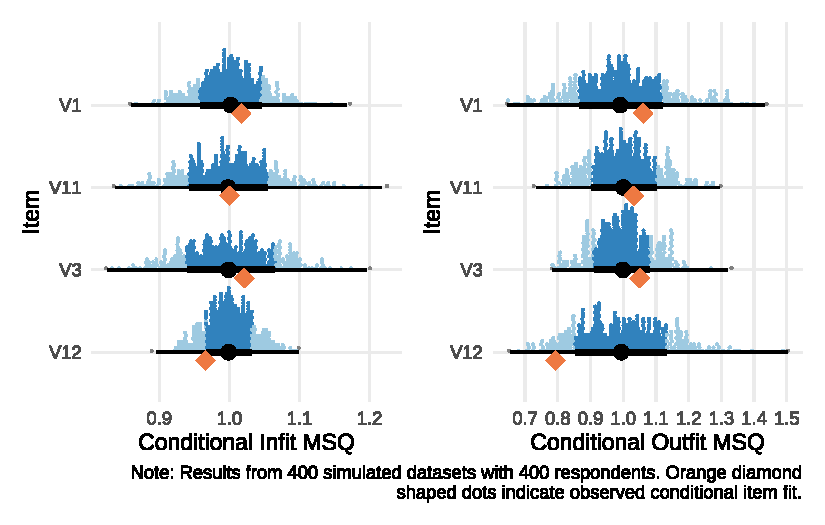
\includegraphics[keepaspectratio]{index_files/figure-pdf/fig-itemfit1-1.pdf}}

}

\caption{\label{fig-itemfit1}Distribution of simulation based item fit
and estimated item fit from observed data}

\end{figure}%

\section{Results}\label{results}

Figures show the percent of simulation runs that have identified an item
as misfitting. Items with more than 5\% are colored in light red. A
number representing the detection rate is shown adjacent to the bar
representing the misfitting item. The figure grid columns are labeled
with the number of iterations used by \texttt{RIgetfit()} to determine
cutoff values and grid rows are labeled with the sample size.

\subsection{Infit}\label{infit}

\phantomsection\label{cell-fig-ifb0}
\begin{figure}[H]

\centering{

\pandocbounded{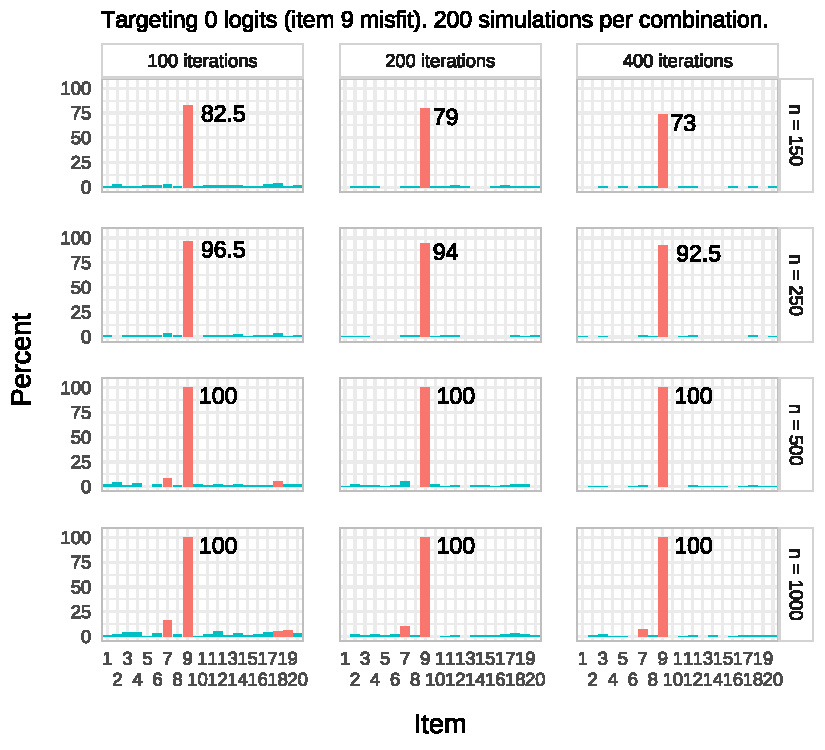
\includegraphics[keepaspectratio]{index_files/figure-pdf/fig-ifb0-1.pdf}}

}

\caption{\label{fig-ifb0}Conditional infit detection rate (misfit item
at 0 logits)}

\end{figure}%

Figure~\ref{fig-ifb0} shows the detection rate when the misfitting item
is located at the sample mean. The detection rate is highest for the
condition with 100 iterations with sample sizes 150 and 250, but it also
shows higher levels of false positives when the sample size increases to
500 or more.

\phantomsection\label{cell-fig-ifb1}
\begin{figure}[H]

\centering{

\pandocbounded{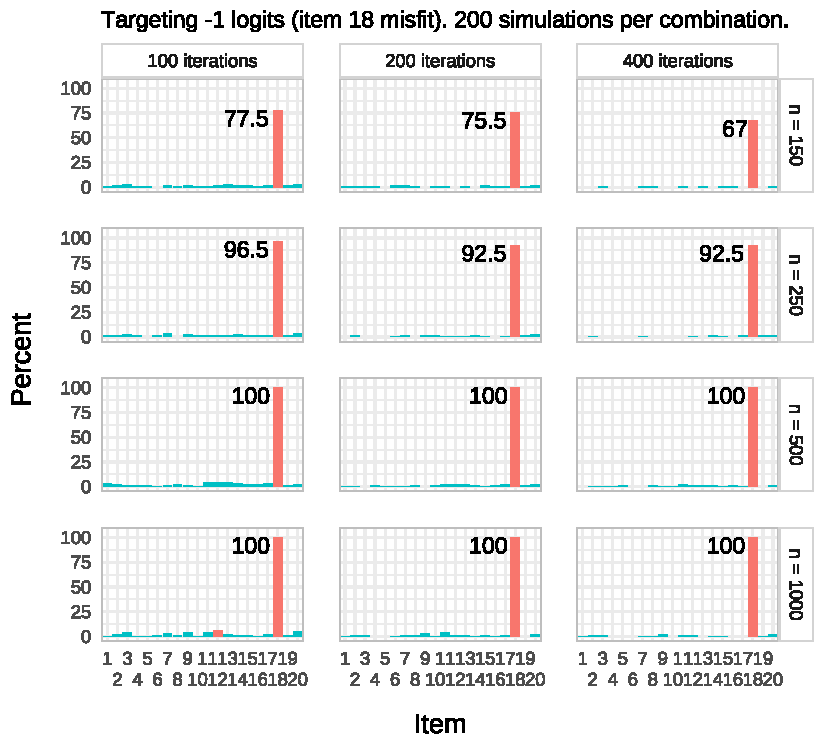
\includegraphics[keepaspectratio]{index_files/figure-pdf/fig-ifb1-1.pdf}}

}

\caption{\label{fig-ifb1}Conditional infit detection rate (misfit item
at -1 logits)}

\end{figure}%

When the misfitting item is offset in targeting by -1 logits compared to
the sample mean (see Figure~\ref{fig-ifb1}), the smallest sample size
has less power to detect misfit compared to the on-target misfitting
item. There are lower rates of false positives across all sample sizes
and iterations.

\phantomsection\label{cell-fig-ifb2}
\begin{figure}[H]

\centering{

\pandocbounded{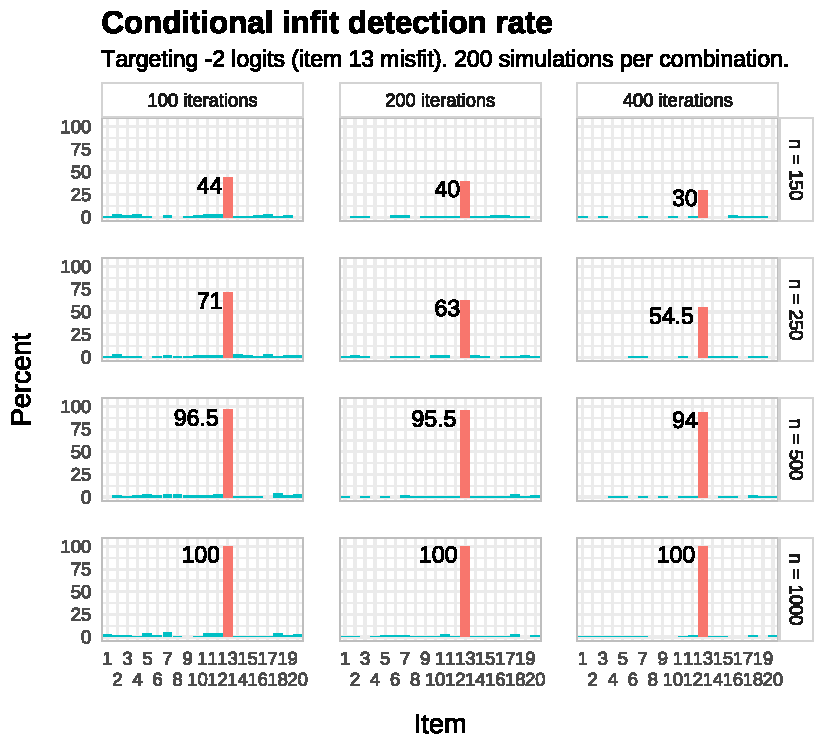
\includegraphics[keepaspectratio]{index_files/figure-pdf/fig-ifb2-1.pdf}}

}

\caption{\label{fig-ifb2}Conditional infit detection rate (misfit item
at -2 logits)}

\end{figure}%

Finally, when the misfitting item is located at -2 logits compared to
the sample mean (see Figure~\ref{fig-ifb2}), we see a stronger reduction
in power for sample sizes 150 and 250. No false positives are
identified.

\subsection{Outfit}\label{outfit}

\phantomsection\label{cell-fig-ifb0out}
\begin{figure}[H]

\centering{

\pandocbounded{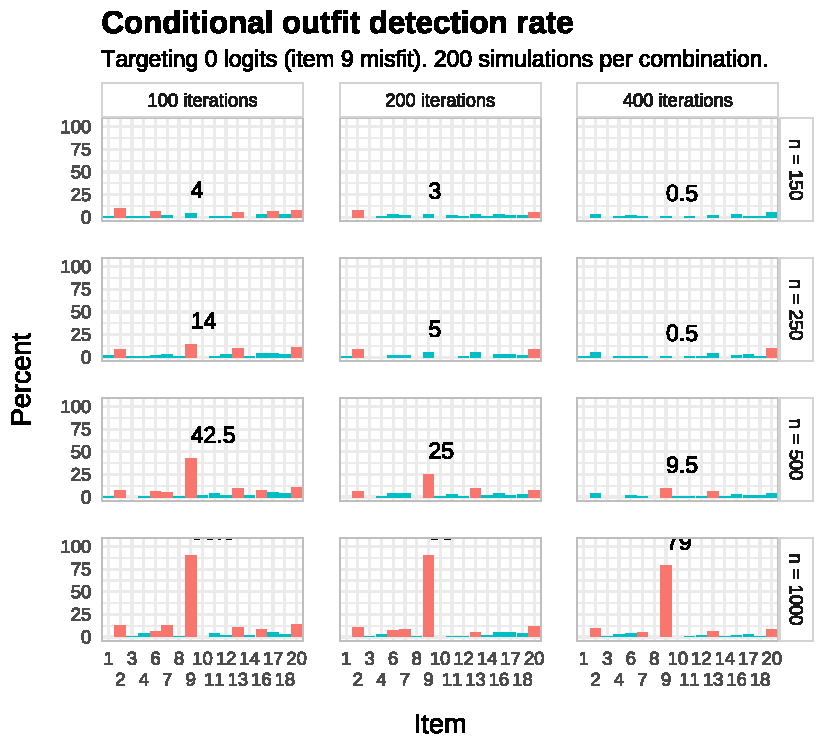
\includegraphics[keepaspectratio]{index_files/figure-pdf/fig-ifb0out-1.pdf}}

}

\caption{\label{fig-ifb0out}Conditional outfit detection rate (misfit
item at 0 logits)}

\end{figure}%

\phantomsection\label{cell-fig-ifb1out}
\begin{figure}[H]

\centering{

\pandocbounded{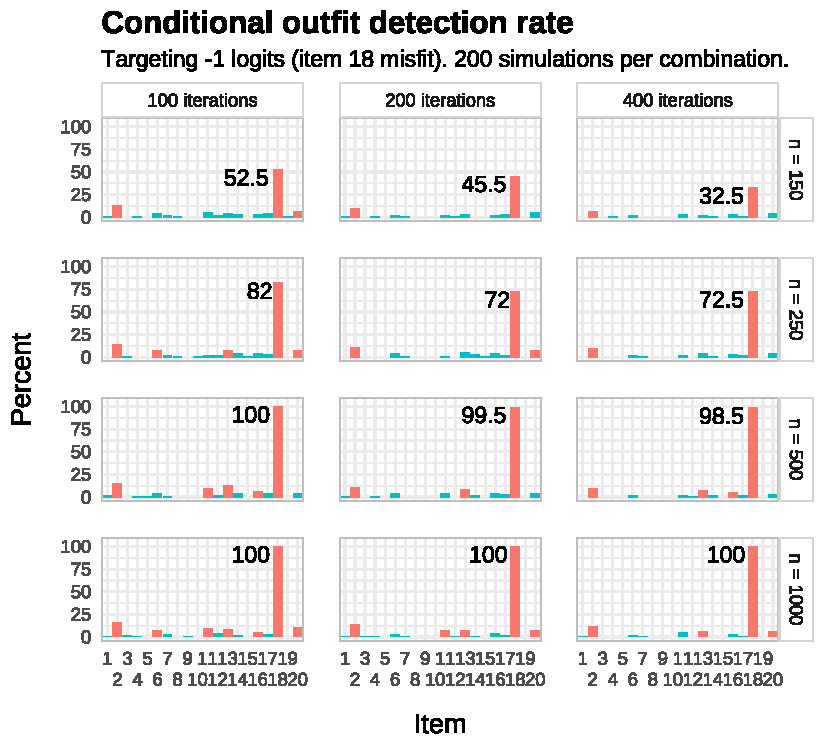
\includegraphics[keepaspectratio]{index_files/figure-pdf/fig-ifb1out-1.pdf}}

}

\caption{\label{fig-ifb1out}Conditional outfit detection rate (misfit
item at -1 logits)}

\end{figure}%

\phantomsection\label{cell-fig-ifb2out}
\begin{figure}[H]

\centering{

\pandocbounded{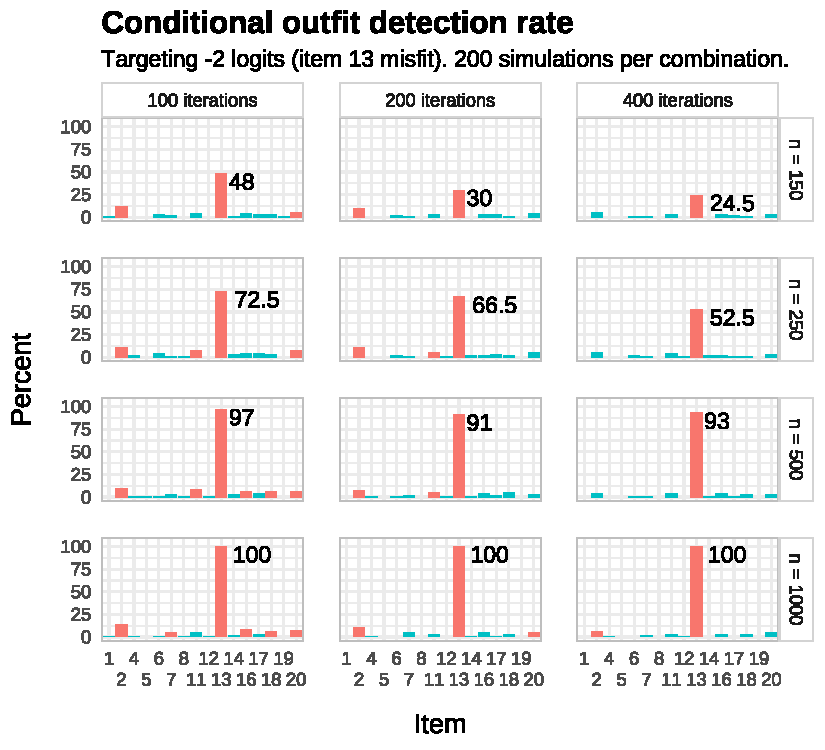
\includegraphics[keepaspectratio]{index_files/figure-pdf/fig-ifb2out-1.pdf}}

}

\caption{\label{fig-ifb2out}Conditional outfit detection rate (misfit
item at -2 logits)}

\end{figure}%

As shown in Figure~\ref{fig-ifb0out}, Figure~\ref{fig-ifb1out}, and
Figure~\ref{fig-ifb2out}, outfit is performing worse than infit across
the board.

\subsection{Comments}\label{comments}

Based on these simulation, it is highly recommended to use infit over
outfit in assessing item fit. The performance of outfit calls to
question whether it is useful at all for detecting item misfit.

Regarding infit and the use of parametric bootstrapping with the
function \texttt{RIgetfit()}, it looks like 100 iterations are to
recommend to determine cutoff values when the sample size is 250 or
lower, while 200 or 400 iterations reduce the risk for false positives
at sample sizes of 500 or larger. False positives are found at sample
sizes 500 and 1000 only. The risk for false positives is notably higher
when the misfitting item is located at the sample mean compared to when
the misfitting item is off-target by -1 logits or more.

Study 2: Item-restscore

Item-restscore is a metric that compares an expected correlation with
the observed correlation, using Goodman and Kruskal's \(\gamma\)
(Goodman and Kruskal 1954; Kreiner 2011). Lower observed values than
expected indicate that an item is underfit to the Rasch model, while
higher values indicate overfit. The item-restscore function used in this
simulation is from the \texttt{iarm} package (Mueller and Santiago 2022)
and outputs Benjamini-Hochberg corrected \emph{p}-values (Benjamini and
Hochberg 1995), which are used to determine whether the differences
between the observed and expected values are statistically significant
(using \emph{p} \textless{} .05 as critical value) for each item. The
data and procedure in this study follow the same structure as Study 1,
with the addition of a smaller sample condition with 100 respondents.

\section{Results}\label{results-1}

\phantomsection\label{cell-fig-itemrestscore1}
\begin{figure}[H]

\centering{

\pandocbounded{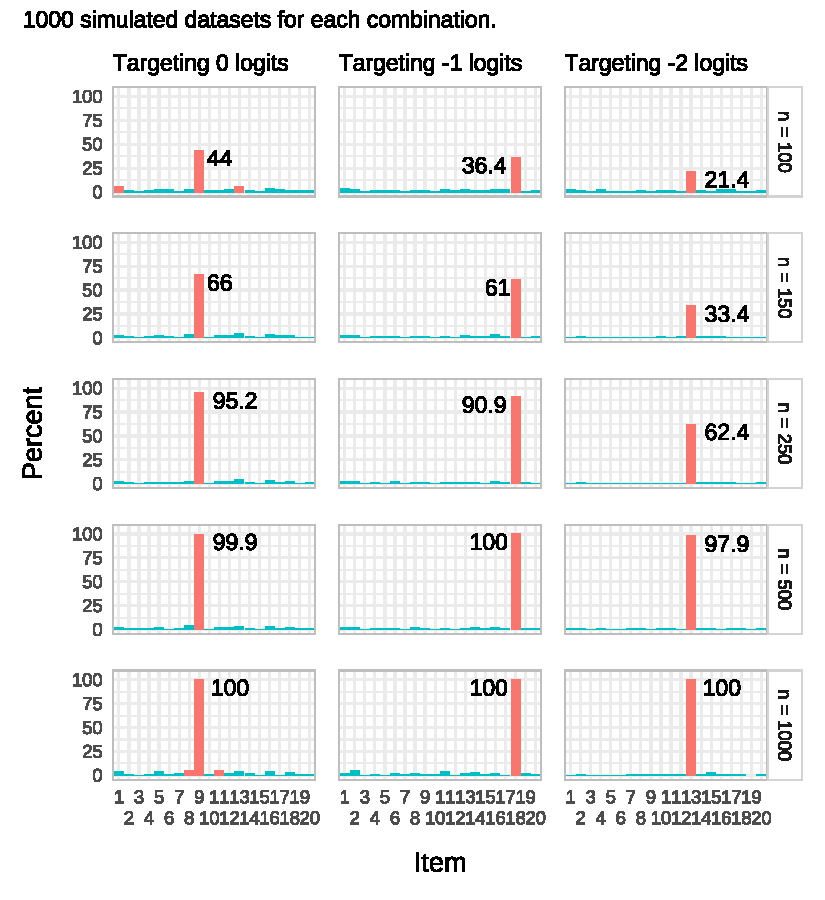
\includegraphics[keepaspectratio]{index_files/figure-pdf/fig-itemrestscore1-1.pdf}}

}

\caption{\label{fig-itemrestscore1}Item-restscore detection rate across
targeting and sample size}

\end{figure}%

This simulation includes an additional condition with 100 respondents,
which results in significantly lower detection rates compared to n =
150. Compared to infit at 250 respondents, item-restscore has detection
rates of 95.2\%, 90.9\%, and 62.4\% for targeting 0, -1, and -2, while
infit has 96.5\%, 96.5\%, and 71\%. For sample sizes 500 and 1000, the
detection rate is similar, including the increased tendency for false
positives at n = 1000. The false positive rate is lower for
item-restscore than infit for sample sizes below 1000.

Study 3: Comparing infit and item-restscore

We will now compare the performance of infit and item-restscore when all
three items are misfitting at the same time. This simulation will also
include a condition with 2000 respondents to examine if the false
positive rate increases with more respondents. For infit, we will use
100 iterations with \texttt{RIgetfit()} for n \textless{} 500 and 200
iterations for n \textgreater= 500 since this produced the best results
in Study 1. Outfit is also included in the study, mostly to check if
its' performance is similar to the condition with only one misfitting
item.

\subsection{Results}\label{results-2}

\phantomsection\label{cell-fig-ifb3out}
\begin{figure}[H]

\centering{

\pandocbounded{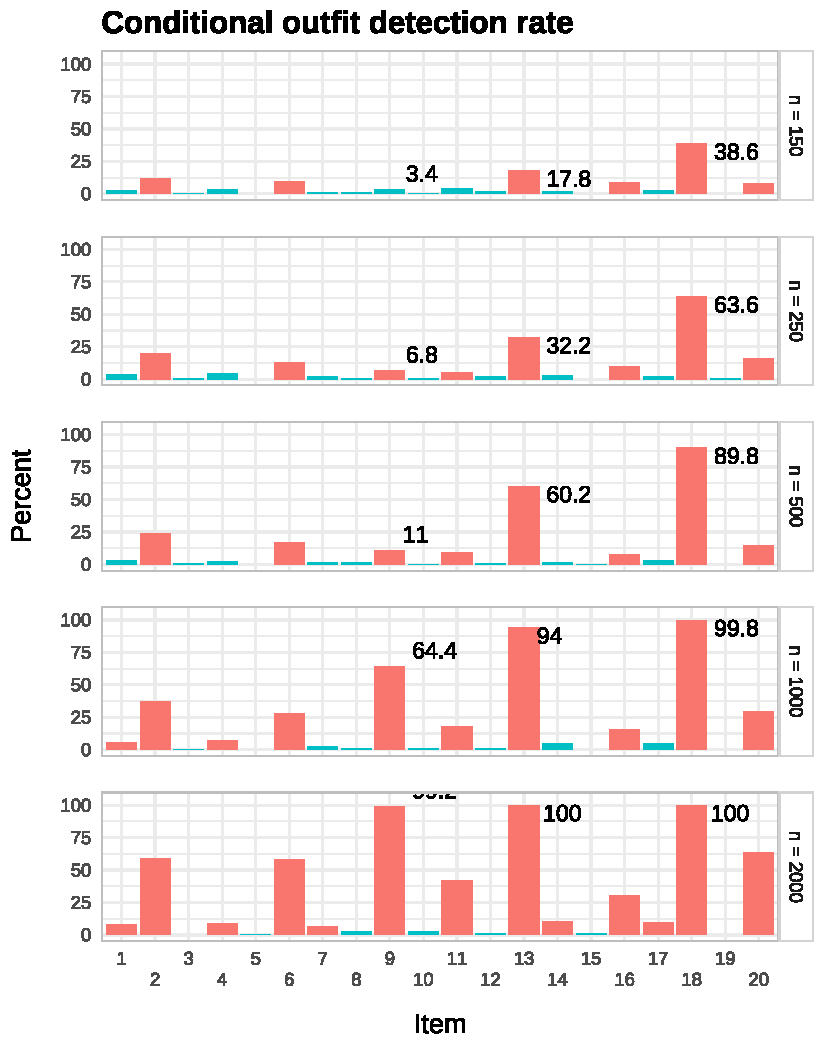
\includegraphics[keepaspectratio]{index_files/figure-pdf/fig-ifb3out-1.pdf}}

}

\caption{\label{fig-ifb3out}Conditional outfit detection rate with three
misfitting items}

\end{figure}%

\phantomsection\label{cell-fig-ifb3}
\begin{figure}[H]

\centering{

\pandocbounded{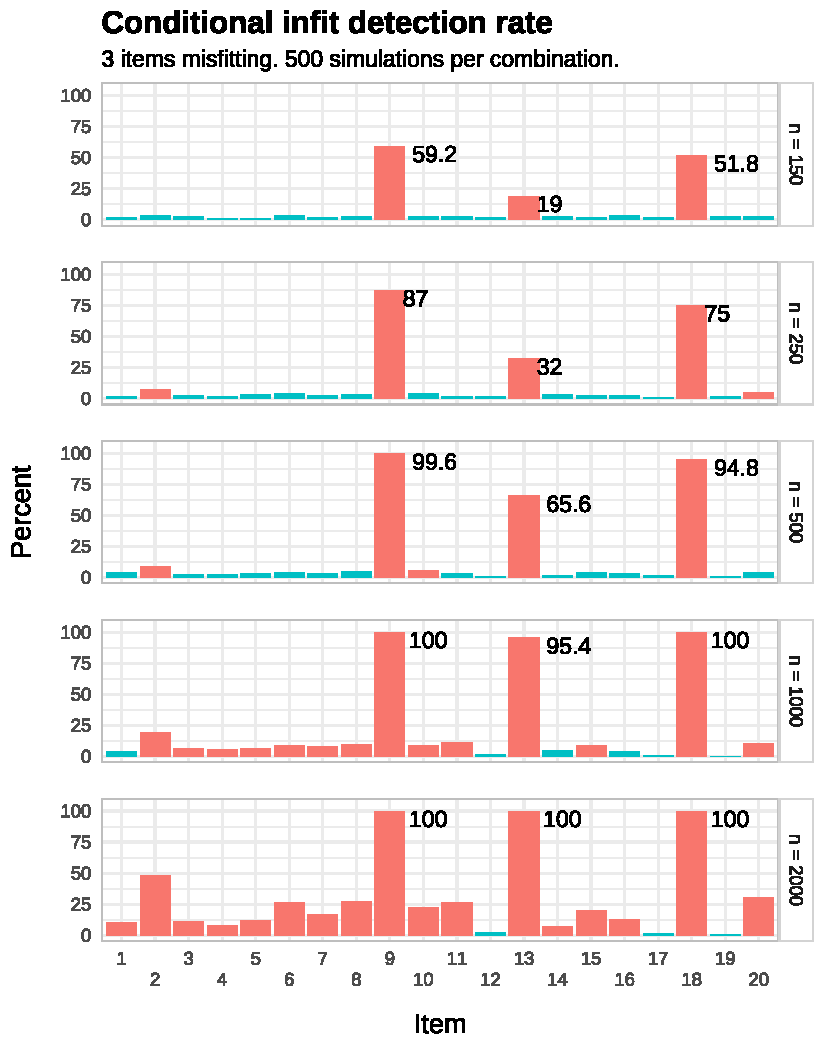
\includegraphics[keepaspectratio]{index_files/figure-pdf/fig-ifb3-1.pdf}}

}

\caption{\label{fig-ifb3}Conditional infit detection rate with three
misfitting items}

\end{figure}%

Looking at the performance of infit with three misfitting items
(Figure~\ref{fig-ifb3}), we can see that the detection rate is markedly
worse for item 13 (targeting -2 logits) in sample sizes 500 and below,
compared to when single items were misfitting. The false positive rate
has increased for a sample size of 1000 and we can see it increase
strongly at n = 2000. Outfit (Figure~\ref{fig-ifb3out}) again performs
worse than infit.

\phantomsection\label{cell-fig-ifb3b}
\begin{figure}[H]

\centering{

\pandocbounded{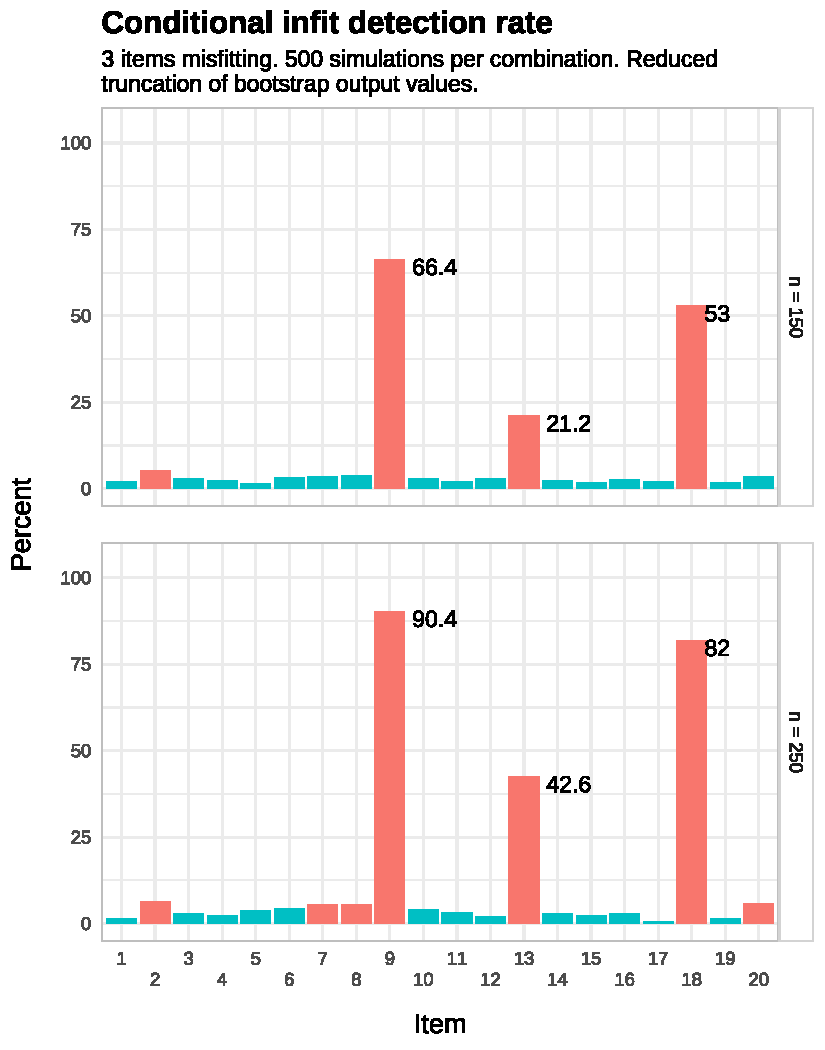
\includegraphics[keepaspectratio]{index_files/figure-pdf/fig-ifb3b-1.pdf}}

}

\caption{\label{fig-ifb3b}Conditional infit detection rate with three
misfitting items}

\end{figure}%

In Figure~\ref{fig-ifb3b}, the minimal truncation used previously to
remove extreme values (quantiles .001 and .999) was increased to .005
and .995. This improves the detection rate, particularly for the n = 250
condition and item 13, but also results in an increased false positive
rate.

\phantomsection\label{cell-fig-itemrestscore2}
\begin{figure}[H]

\centering{

\pandocbounded{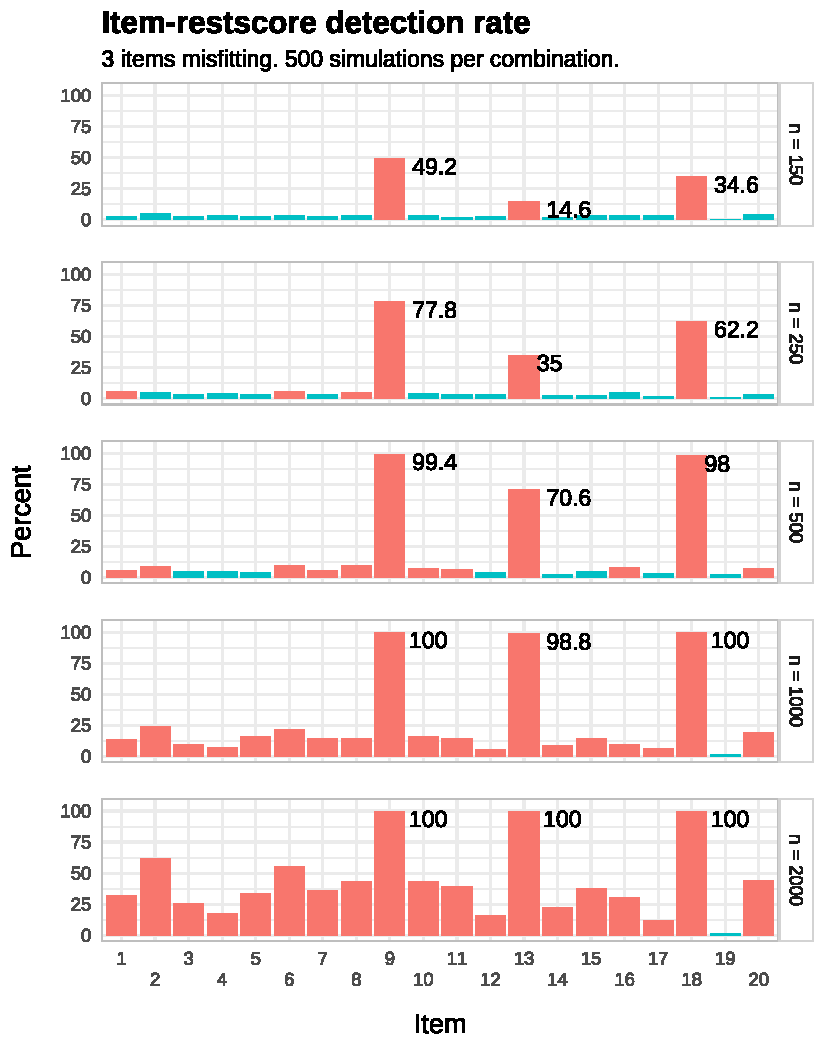
\includegraphics[keepaspectratio]{index_files/figure-pdf/fig-itemrestscore2-1.pdf}}

}

\caption{\label{fig-itemrestscore2}}

\end{figure}%

\phantomsection\label{cell-fig-comp1}
\begin{figure}[H]

\centering{

\pandocbounded{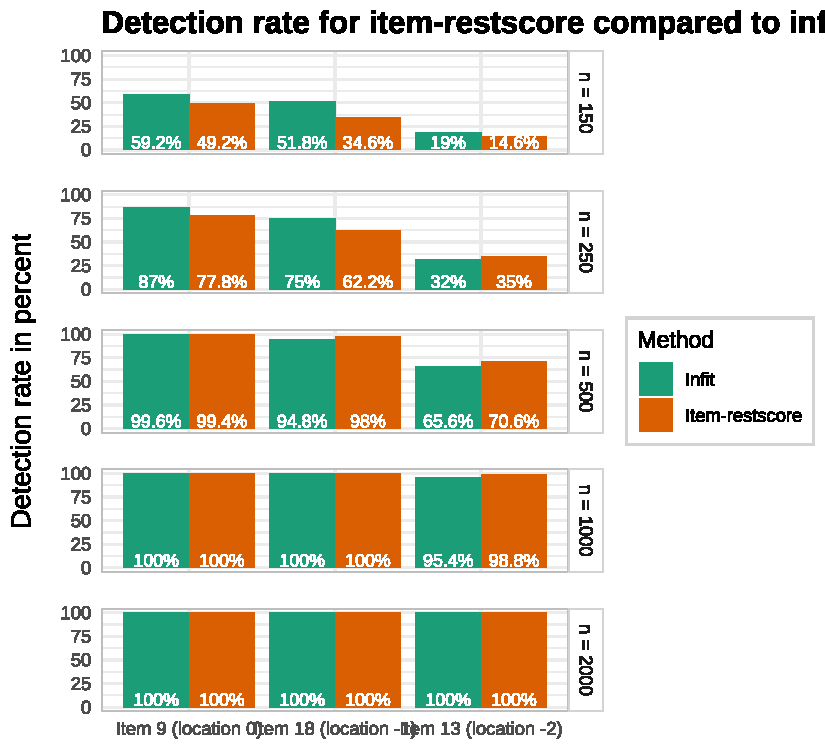
\includegraphics[keepaspectratio]{index_files/figure-pdf/fig-comp1-1.pdf}}

}

\caption{\label{fig-comp1}Detection rate for item-restscore compared to
infit}

\end{figure}%

Item-restscore (see Figure~\ref{fig-itemrestscore2}) shows a comparable
detection rate to infit and higher levels of false positives. A
comparison is made between the two in Figure~\ref{fig-comp1}, where
item-restscore is performing better than infit at detecting the -2
logits off-target item at n = 250, and better across all items for n =
500 and n = 1000. Infit performs better for samples n = 150 and n = 250
(except for the item with location -2 logits).

\begin{longtable}[]{@{}
  >{\raggedleft\arraybackslash}p{(\linewidth - 4\tabcolsep) * \real{0.4300}}
  >{\raggedright\arraybackslash}p{(\linewidth - 4\tabcolsep) * \real{0.2900}}
  >{\raggedleft\arraybackslash}p{(\linewidth - 4\tabcolsep) * \real{0.2900}}@{}}

\caption{\label{tbl-overunder}Item-restscore summary results across all
sample sizes}

\tabularnewline

\toprule\noalign{}
\begin{minipage}[b]{\linewidth}\raggedleft
Item
\end{minipage} & \begin{minipage}[b]{\linewidth}\raggedright
Type of misfit
\end{minipage} & \begin{minipage}[b]{\linewidth}\raggedleft
Percent
\end{minipage} \\
\midrule\noalign{}
\endhead
\bottomrule\noalign{}
\endlastfoot
9 & underfit & 85.28 \\
18 & underfit & 78.96 \\
13 & underfit & 63.80 \\
2 & overfit & 20.80 \\
6 & overfit & 19.00 \\
20 & overfit & 15.48 \\
8 & overfit & 15.28 \\
10 & overfit & 14.60 \\
11 & overfit & 13.04 \\
7 & overfit & 12.52 \\
15 & overfit & 12.52 \\
1 & overfit & 11.96 \\
5 & overfit & 11.92 \\
16 & overfit & 11.12 \\
3 & overfit & 8.96 \\
14 & overfit & 7.28 \\
4 & overfit & 7.24 \\
12 & overfit & 5.96 \\
17 & overfit & 5.16 \\
19 & overfit & 1.24 \\
12 & underfit & 0.08 \\

\end{longtable}

Reviewing the type of misfit identified by item-restscore (see
Table~\ref{tbl-overunder}), the false positives are all overfitting the
Rasch model, except for two instances (out of 2500) indicating underfit
for item 12. Items 9, 13, and 18, which were simulated to be misfitting
due to loading on a separate dimension, are as expected showing underfit
to the Rasch model.

Study 4: Bootstrapped item-restscore

For this set of simulations, we will use a non-parametric bootstrap
procedure with item-restscore. The difference from the parametric
bootstrap is that the non-parametric bootstrap samples with replacement
directly from the observed response data. First, based on the above
problematic sample size of 2000 when three items are misfitting, we will
use the bootstrap function to sample with replacement using n = 800 and
250 bootstrap samples. The function \texttt{RIbootRestscore()} from the
\texttt{easyRasch} package will be used.

\begin{longtable}[]{@{}
  >{\raggedright\arraybackslash}p{(\linewidth - 4\tabcolsep) * \real{0.4300}}
  >{\raggedright\arraybackslash}p{(\linewidth - 4\tabcolsep) * \real{0.2900}}
  >{\raggedleft\arraybackslash}p{(\linewidth - 4\tabcolsep) * \real{0.2900}}@{}}

\caption{\label{tbl-bootir}Example output from
\texttt{RIbootRestscore()}}

\tabularnewline

\toprule\noalign{}
\begin{minipage}[b]{\linewidth}\raggedright
Item
\end{minipage} & \begin{minipage}[b]{\linewidth}\raggedright
Item-restscore result
\end{minipage} & \begin{minipage}[b]{\linewidth}\raggedleft
Percent of iterations
\end{minipage} \\
\midrule\noalign{}
\endhead
\bottomrule\noalign{}
\endlastfoot
V9 & underfit & 100.0 \\
V18 & underfit & 99.6 \\
V13 & underfit & 96.8 \\
V2 & overfit & 67.2 \\
V10 & overfit & 36.8 \\
V6 & overfit & 35.2 \\
V7 & overfit & 23.6 \\
V5 & overfit & 19.6 \\
V8 & overfit & 18.0 \\
V15 & overfit & 17.2 \\
V4 & overfit & 13.2 \\
V16 & overfit & 9.6 \\
V11 & overfit & 8.4 \\
V20 & overfit & 7.6 \\
V1 & overfit & 6.4 \\
V3 & overfit & 4.4 \\
V17 & overfit & 3.6 \\
V14 & overfit & 1.6 \\
V19 & overfit & 1.2 \\
V12 & overfit & 0.4 \\
V3 & underfit & 0.4 \\

\end{longtable}

\texttt{RIbootRestscore()} is demonstrated using a single sample in
Table~\ref{tbl-bootir}, where the table is sorted on the percent of
iterations. The runtime was approximately 10-12 seconds using 8 CPU
cores on a Macbook Pro M1 Max. In the simulation, we will repeat this
procedure 500 times and report the average and standard deviation for
the percent indicating misfit for each item.

Second, we will also apply the bootstrapped item-restscore method to
sample sizes 150 and 250, using the complete sample for the same
bootstrap procedure to see if this produces more useful information than
previously tested strategies for identifying misfitting items.

\section{Results}\label{results-3}

\phantomsection\label{cell-fig-irb0all}
\begin{figure}[H]

\centering{

\pandocbounded{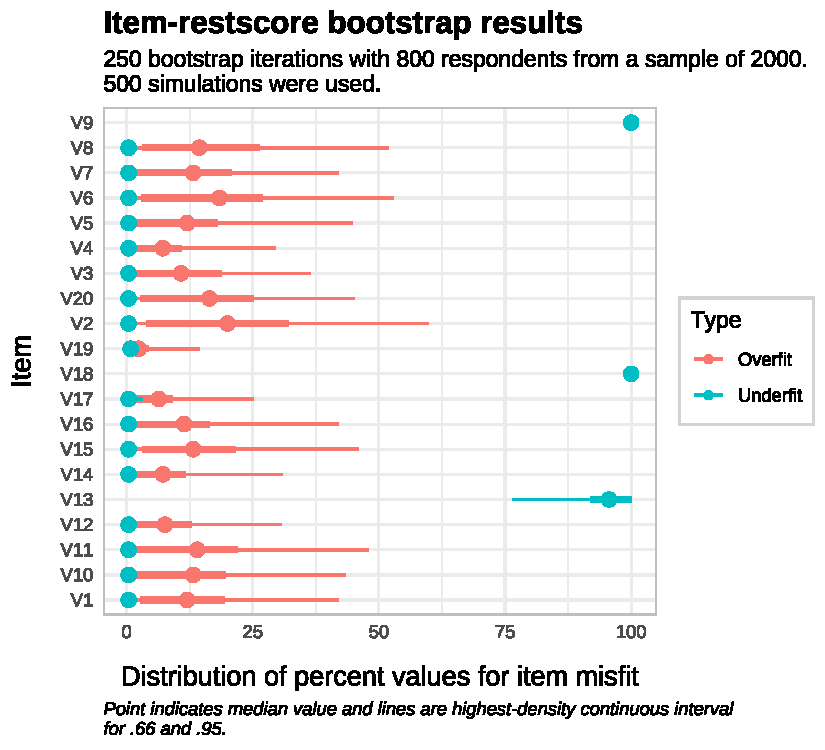
\includegraphics[keepaspectratio]{index_files/figure-pdf/fig-irb0all-1.pdf}}

}

\caption{\label{fig-irb0all}Item-restscore bootstrap results}

\end{figure}%

\begin{table}

\caption{\label{tbl-irb0mis}Summary statistics for item-restscore
bootstrap simulation}

\begin{minipage}{\linewidth}

\subcaption{\label{tbl-irb0mis-1}Misfitting items}

\centering{

\begin{tabular}{lrrrrr}
\toprule
Item & Median & MAD & Mean & SD & Percentile .05\\
\midrule
V9 & 100.0 & 0.0 & 100.0 & 0.1 & 100.0\\
V18 & 100.0 & 0.0 & 99.8 & 0.9 & 99.2\\
V13 & 95.6 & 4.7 & 93.0 & 8.0 & 76.4\\
\bottomrule
\end{tabular}

}

\end{minipage}%
\newline
\begin{minipage}{\linewidth}

\subcaption{\label{tbl-irb0mis-2}False positives}

\centering{

\begin{tabular}{lrrrrr}
\toprule
Item & Median & MAD & Mean & SD & Percentile .95\\
\midrule
V2 & 20.0 & 15.4 & 24.3 & 16.7 & 58.8\\
V6 & 18.4 & 14.2 & 21.3 & 14.9 & 52.8\\
V8 & 14.4 & 12.5 & 19.7 & 15.6 & 51.6\\
V11 & 14.0 & 11.9 & 17.6 & 13.9 & 47.7\\
V15 & 13.2 & 10.1 & 16.6 & 13.4 & 45.2\\
V20 & 16.4 & 13.6 & 19.5 & 13.9 & 45.2\\
V5 & 12.0 & 10.1 & 15.7 & 12.6 & 44.4\\
V10 & 13.2 & 11.3 & 16.4 & 13.0 & 42.4\\
V16 & 11.4 & 10.4 & 15.2 & 13.0 & 42.0\\
V7 & 13.2 & 11.9 & 16.7 & 12.6 & 41.6\\
V1 & 12.0 & 10.1 & 15.5 & 12.8 & 41.3\\
V3 & 10.8 & 9.5 & 13.6 & 11.2 & 36.1\\
V14 & 7.2 & 6.5 & 10.4 & 10.1 & 30.7\\
V12 & 7.6 & 7.7 & 10.4 & 9.5 & 29.7\\
V4 & 7.2 & 6.5 & 10.2 & 9.5 & 29.3\\
V17 & 6.4 & 6.5 & 8.4 & 8.0 & 24.4\\
V19 & 2.4 & 2.4 & 3.9 & 4.6 & 13.6\\
\bottomrule
\end{tabular}

}

\end{minipage}%

\end{table}%

Figure~\ref{fig-irb0all} shows that there is variation in the false
positive rate and it is nearly always indicating overfit, while the
misfitting items are only indicated as underfit. The summary statistics
in Table~\ref{tbl-irb0mis} show that there can be quite a bit of
variation for false positives, but the clear majority of results are
below 50\%. 3 items have 95th percentile values above 50, with the
highest at 58.8.

\section{Small sample (n = 150)}\label{small-sample-n-150}

We will use 200 simulations to check the performance of the bootstrapped
item-restscore function for sample size 150. As an additional
experimental condition, we will use both 250 and 500 bootstrap
iterations for item-restscore in each simulation.

\phantomsection\label{cell-fig-irboot150}
\begin{figure}[H]

\centering{

\pandocbounded{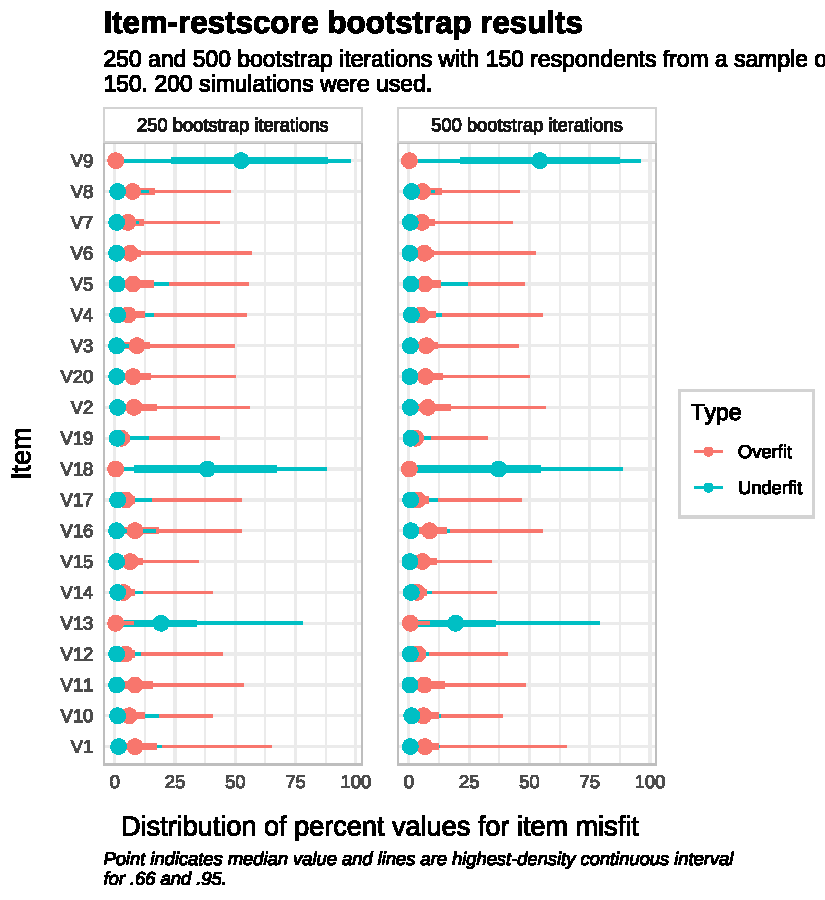
\includegraphics[keepaspectratio]{index_files/figure-pdf/fig-irboot150-1.pdf}}

}

\caption{\label{fig-irboot150}}

\end{figure}%

Item-restscore bootstrapping improves slightly on the single instance of
item-restscore for the n = 150 condition (see
Figure~\ref{fig-irboot150}). When comparing to the previous results in
Figure~\ref{fig-itemrestscore2}, where the detection rate for the same
sample size was at 49.2\%, 14.6\%, and 34.6\% (for items 9, 13, and 18
respectively), the corresponding median values from the bootstrapped
item-restscore with 250 iterations were 52.4\%, 19.2\%, and 38.4\%.
Using 500 bootstrap iterations did not result in relevant improvements
over 250 iterations (see Table~\ref{tbl-irb150mis}). Compared to the
results using infit (Figure~\ref{fig-ifb3}), with detection rates of
59.2\%, 19\%, and 51.8\%, item-restscore inferior also when
bootstrapped.

\begin{longtable}[]{@{}llrrrr@{}}

\caption{\label{tbl-irb150mis}Summary statistics for item-restscore
bootstrap simulation (n = 150)}

\tabularnewline

\toprule\noalign{}
Bootstrap iterations & Item & Median & MAD & Mean & SD \\
\midrule\noalign{}
\endhead
\bottomrule\noalign{}
\endlastfoot
& V9 & 52.4 & 38.0 & 51.4 & 29.2 \\
250 & V18 & 38.4 & 35.6 & 42.0 & 27.8 \\
& V13 & 19.2 & 21.9 & 27.3 & 25.0 \\
& V9 & 54.3 & 37.8 & 51.0 & 29.5 \\
500 & V18 & 37.2 & 35.9 & 41.4 & 27.9 \\
& V13 & 19.4 & 23.1 & 27.2 & 24.7 \\

\end{longtable}

Study 5: Varying the number of items

When doing simulation studies there is always a balance to strike
between trying to evaluate many scenarios and not having too high
complexity. We have been keeping several things constant, such as item
locations and number of items, which makes interpretation easier but may
limit the applicability of the results. For our final simulation, we
will vary the number of items and the number of misfitting items. First,
40 dichotomous items will be used, adding 20 new item locations to the
previously used set, with the same three items misfitting (items 9, 13,
and 18). Second, items 1-10 out of the initial 20 items will be used,
which means only item 9 will be misfit. We'll again be using sample
sizes of 150, 250, 500, and 1000.

Item-restscore and item infit will be compared. The latter will use 100
bootstrap iterations to determine critical values for sample sizes 150
and 250, and 200 bootstrap iterations for n \textgreater= 500.

\section{Results 40 items}\label{results-40-items}

\phantomsection\label{cell-fig-ifb40}
\begin{figure}[H]

\centering{

\pandocbounded{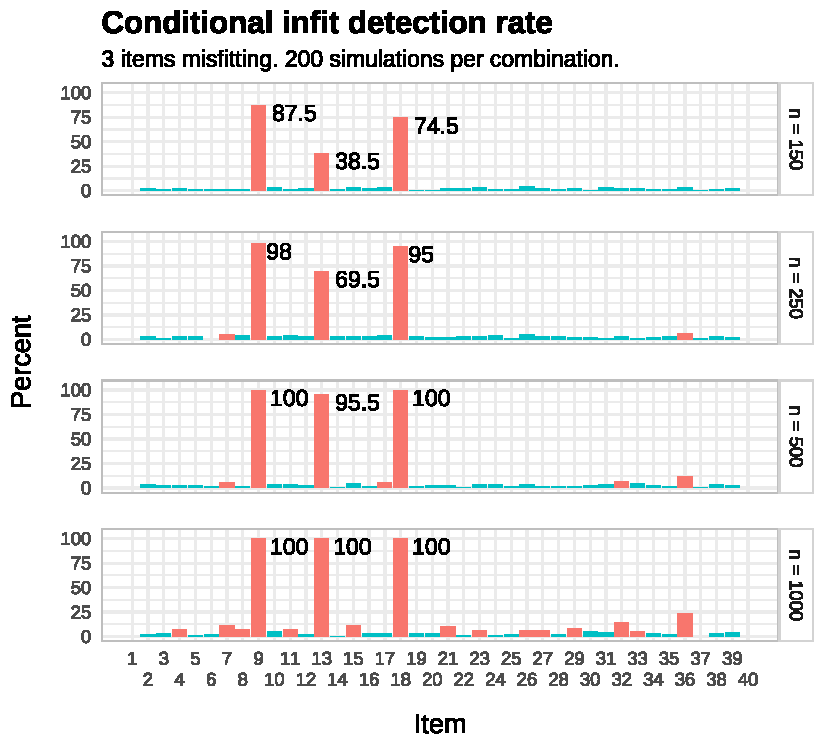
\includegraphics[keepaspectratio]{index_files/figure-pdf/fig-ifb40-1.pdf}}

}

\caption{\label{fig-ifb40}}

\end{figure}%

\phantomsection\label{cell-fig-itemrestscore40}
\begin{figure}[H]

\centering{

\pandocbounded{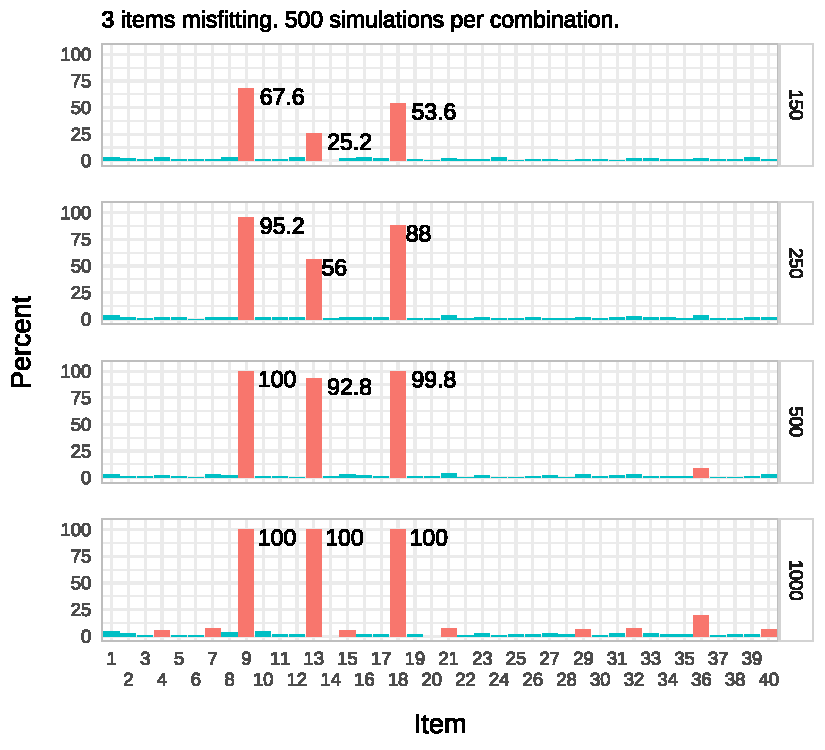
\includegraphics[keepaspectratio]{index_files/figure-pdf/fig-itemrestscore40-1.pdf}}

}

\caption{\label{fig-itemrestscore40}}

\end{figure}%

Infit performs better when the sample size is 150 or 250 (see
Figure~\ref{fig-ifb40}), while performance is slightly better for
item-restscore for n \textgreater= 500 in terms of lower rates of false
positives (see Figure~\ref{fig-itemrestscore40}).

\section{Results 10 items}\label{results-10-items}

\phantomsection\label{cell-fig-ifb10}
\begin{figure}[H]

\centering{

\pandocbounded{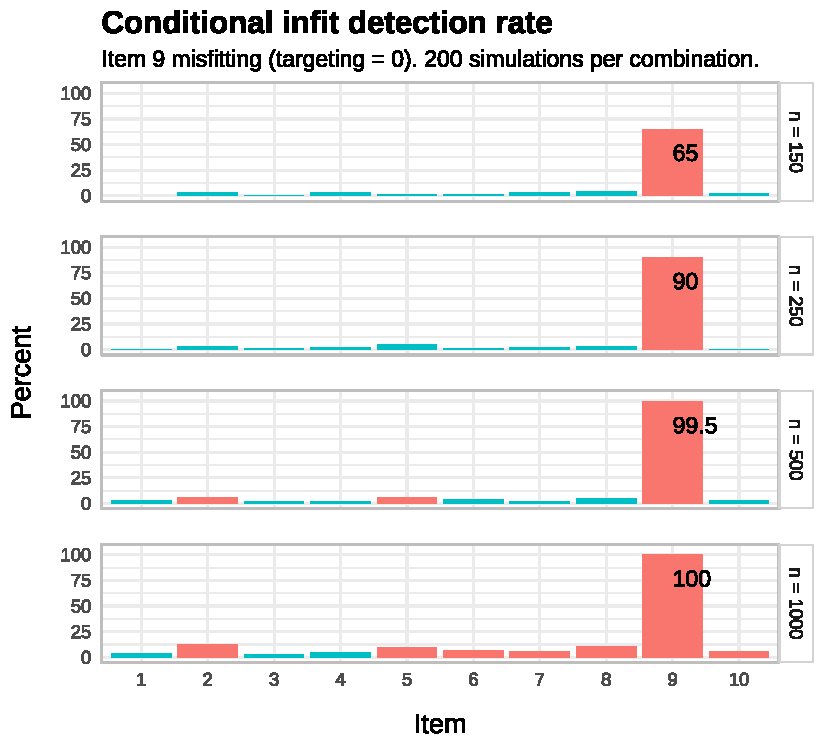
\includegraphics[keepaspectratio]{index_files/figure-pdf/fig-ifb10-1.pdf}}

}

\caption{\label{fig-ifb10}}

\end{figure}%

\phantomsection\label{cell-fig-itemrestscore10}
\begin{figure}[H]

\centering{

\pandocbounded{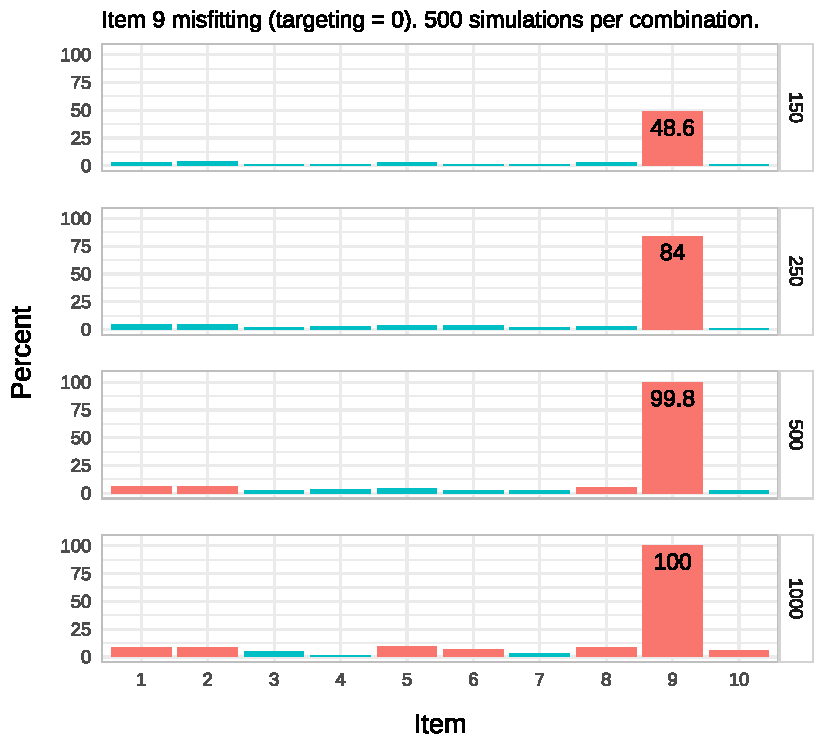
\includegraphics[keepaspectratio]{index_files/figure-pdf/fig-itemrestscore10-1.pdf}}

}

\caption{\label{fig-itemrestscore10}}

\end{figure}%

\section{Summary figure}\label{summary-figure}

\phantomsection\label{cell-fig-comp10}
\begin{figure}[H]

\centering{

\pandocbounded{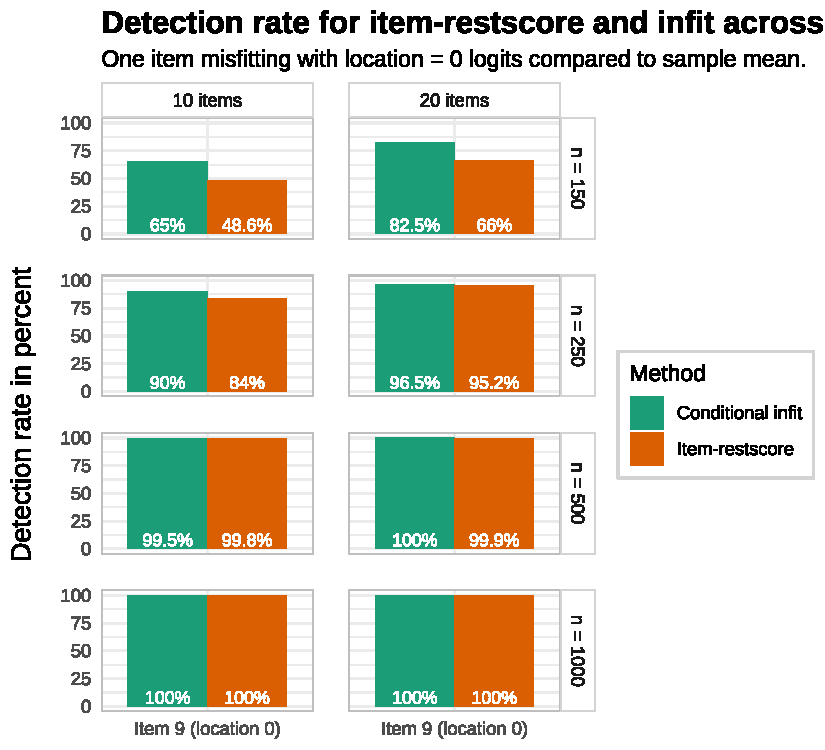
\includegraphics[keepaspectratio]{index_files/figure-pdf/fig-comp10-1.pdf}}

}

\caption{\label{fig-comp10}Detection rate for item-restscore and infit
for 10 items}

\end{figure}%

\phantomsection\label{cell-fig-comp2040}
\begin{verbatim}
List of 1
 $ axis.title.x: list()
  ..- attr(*, "class")= chr [1:2] "element_blank" "element"
 - attr(*, "class")= chr [1:2] "theme" "gg"
 - attr(*, "complete")= logi FALSE
 - attr(*, "validate")= logi TRUE
\end{verbatim}

\begin{figure}[H]

\centering{

\pandocbounded{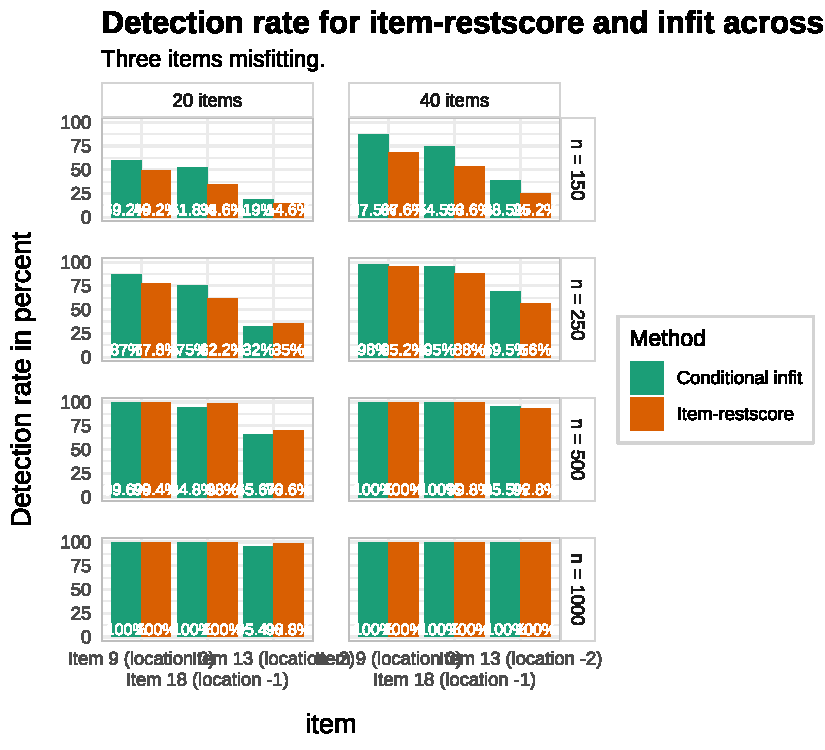
\includegraphics[keepaspectratio]{index_files/figure-pdf/fig-comp2040-1.pdf}}

}

\caption{\label{fig-comp2040}Detection rate for item-restscore and infit
for 20 and 40 items}

\end{figure}%

Figure~\ref{fig-comp10} and Figure~\ref{fig-comp2040} summarize the
findings from the two different comparisons of item numbers. Adding more
items improves the detection rate substantially for both methods,
particularly for smaller samples and the off-target items. 40 items
compared to 20 items result in a larger improvement for infit over
item-restscore for the n = 150 condition, but also the n = 250 and n =
500 conditions for the -2 logits off-target item.

Study 6: Conditional likelihood ratio test

While global tests of model fit don't provide any information about
reasons for misfit when detected, they can be useful together with more
specific tests such as those demonstrated in this paper. A commonly used
global goodness-of-fit test is the Likelihood Ratio Test (LRT, Andersen
1973), which is also implemented in the \texttt{eRm} package. While the
global test is not central to the purposes of this paper (detecting item
misfit), it could provide readers with a familiar test as a reference
and perhaps aid the item-focused methods in determining misfit. Previous
simulation studies evaluating the LRT have found it to not be sensitive
to detect multidimensionality (Debelak 2019).

For this simulation, sample sizes were set to 150, 250, 500, 1000, and
2000, using 1000 simulations for each condition. Study 6 follows the
previous procedures. First, the three datasets with one misfitting item
out of 20, varying the misfitting items location (0, -1, and -2 logits).
Then the datasets with three misfitting items, and comparing 20 and 40
items. And finally, one dataset with 10 items and one well-targeted
misfitting item.

\section{Results}\label{results-4}

\begin{figure}

\begin{minipage}{\linewidth}

\centering{

\pandocbounded{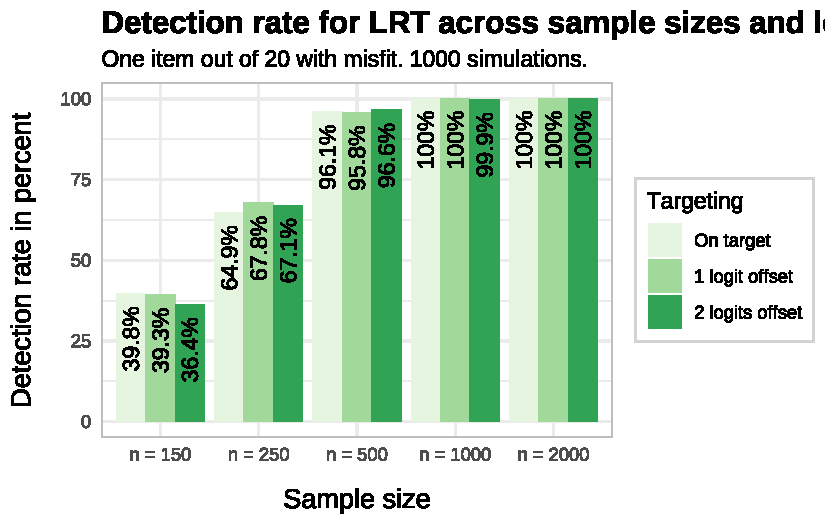
\includegraphics[keepaspectratio]{index_files/figure-pdf/fig-lrt1-1.pdf}}

}

\subcaption{\label{fig-lrt1-1}Across sample sizes and location of misfit
item}

\end{minipage}%
\newline
\begin{minipage}{\linewidth}

\centering{

\pandocbounded{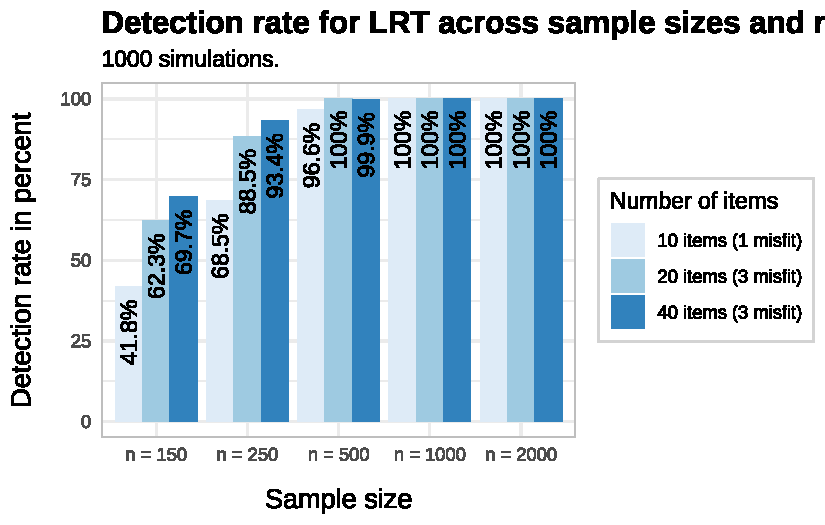
\includegraphics[keepaspectratio]{index_files/figure-pdf/fig-lrt1-2.pdf}}

}

\subcaption{\label{fig-lrt1-2}Across sample sizes and number of items}

\end{minipage}%

\caption{\label{fig-lrt1}Likelihood ratio test detection rate}

\end{figure}%

Results for targeting of the misfit item are summarized in
Figure~\ref{fig-lrt1}, where the detection rate is reported based on the
proportion of p-values below .05 in each condition.

LRT performs better than item-restscore for the off-target item
conditions, especially when targeting was at -2 logits. Otherwise,
performance is similar. Infit is better than LRT for n \textless{} 500
when targeting = 0, similar at targeting = 1, and LRT is better than
infit at targeting -2.

Looking at LRT for different numbers of items and comparing to results
for infit and item-restscore at their best detection rates for the
corresponding number of items and sample size, it shows much worse
performance for 10 items compared to infit and item-restscore at n =
150, but similar performance at larger sample sizes. For 20 and 40
items, LRT is similar to infit at all sample sizes, and slightly better
than item-restscore for n \textless{} 500.

Discussion

This paper was created primarily out of a desire to understand the
performance of conditional item fit and item-restscore in detecting item
misfit. Studies 1-3 and 5 were originally planned, while study 4 was
added due to the results of previous studies showing issues with large
sample sizes, and study 6 was added mostly for didactic purposes but
also out of curiosity of the global fit LRT performance compared to the
other methods. Müller's (2020) paper on conditional item fit was
published five years ago with results that should have sparked
discussions in the Rasch community about updating methods (and software)
and the justification of rule-of-thumb critical values. We hope that
this paper can help spur such discussions by the simple methodology and
presentation of results used, which could make this paper more
accessible for practitioners.

Main results summarized:

\begin{itemize}
\tightlist
\item
  small samples (n \textless{} 250-500) with small numbers of items make
  it harder to detect misfitting items
\item
  small samples (n \textless{} 250-500) should rely primarily on
  conditional item infit with simulation-based critical values
\item
  large samples (n \textgreater{} 500) should use bootstrapped
  item-restscore to reduce the risk of falsely identifying misfit
\item
  misfit in an off-target item is harder to detect than well-targeted
  items and the LRT test can assist in identifying misfit in off-target
  items
\item
  increased number of items increases the power to detect misfit
\end{itemize}

Assessment of item fit and dimensionality should always be done using
multiple methods. Study 6 showed the benefits of also looking at the
likelihood ratio test when the misfitting item is located -2 logits away
from the sample mean location. Previous simulation studies concluded
that the LRT did not perform well at detecting multidimensionality,
which is how the misfitting items were generated in this study. While no
method in this study achieved very good results at the lowest sample
size (n = 150), LRT did not do much worse than the other methods.

\phantomsection\label{cell-fig-loadloc}
\begin{figure}[H]

\centering{

\pandocbounded{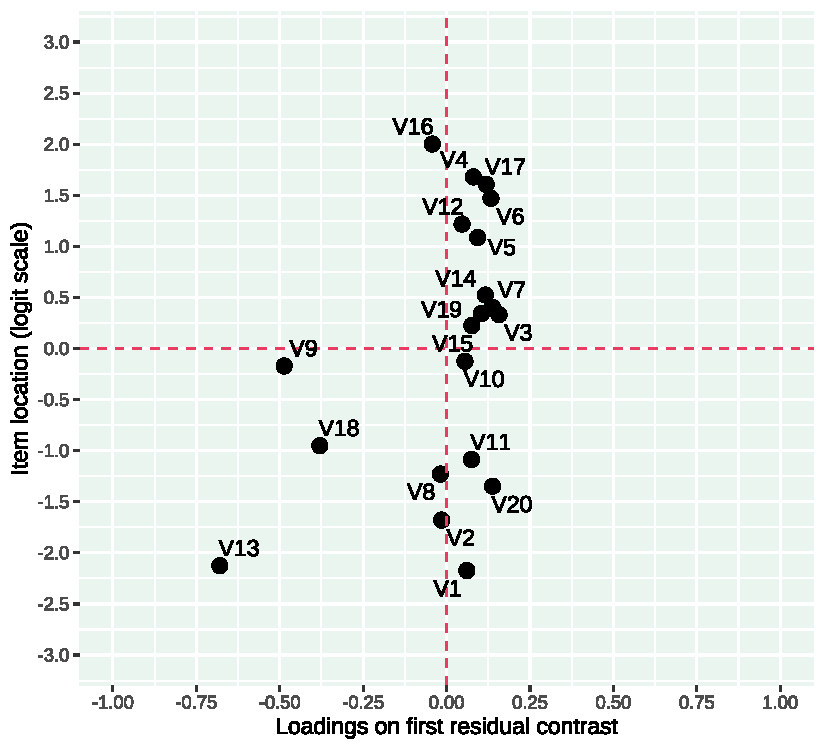
\includegraphics[keepaspectratio]{index_files/figure-pdf/fig-loadloc-1.pdf}}

}

\caption{\label{fig-loadloc}}

\end{figure}%

Item fit and item-restscore are recommended to be used in parallel,
while also examining residual patterns by reviewing standardized factor
loadings on the first residual contrast (see Figure~\ref{fig-loadloc}
for an example using n = 400) as well as Yen's Q3 residual correlations
(Christensen, Makransky, and Horton 2017). Regarding residual
correlations and critical values, the \texttt{easyRasch} package also
contains a function to use bootstrapping (\texttt{RIgetResidCor()}),
similar to the \texttt{RIgetfit()} function, to determine the
appropriate cutoff. This is described briefly in a blog post (Johansson
2024b) and a simulation paper is under preparation.

Item fit in this paper has been assessed using data from individual
respondent residuals in a sample. A useful additional method to evaluate
and understand item fit or misfit is to inspect item characteristic
curves where the sample is divided into class intervals based on their
total score (Buchardt, Christensen, and Jensen 2023) and the group
residuals are inspected.

While the simulations in this paper have all used dichotomous data, all
functions evaluated from the \texttt{easyRasch} package in this paper
also work with polytomous data using the Rasch Partial Credit Model.

\section{Limitations}\label{limitations}

The total number of items and the proportion of misfit items clearly
have effects on detection rate and could have been investigated further
using more variations in sample sizes. The Rasch partial credit model
for polytomous data (PCM, Masters 1982) would have been useful to
include in a comparison study. When testing the bootstrapped
item-restscore method, more variations in the number of bootstrap
samples (iterations) might have been of interest, although the
difference between 250 and 500 was small.

Conclusion

For sample sizes under 500, it seems best to rely mostly on item infit
with simulation-based critical values, using 100 iterations with
\texttt{RIgetfit()}. For sample sizes closer to 500, item-restscore is
recommended as the primary method, either as a single-run test or
bootstrapped. With samples larger than 500, bootstrapped item-restscore
controls false positive rates well, while showing high rates of misfit
detection. Using 250 iterations for the bootstrapped item-restscore
seems adequate. In general, both infit and item-restscore are useful in
the analysis process if you have a sample size below 1000.

The findings reported here also make a good argument for removing one
item at a time when the analysis indicates several misfitting items,
starting with the most underfitting item. This is especially relevant
for n \textgreater= 500 and when misfitting items are located close to
the sample mean.

References

\phantomsection\label{refs}
\begin{CSLReferences}{1}{0}
\bibitem[\citeproctext]{ref-andersen_goodness_1973}
Andersen, Erling B. 1973. {``A Goodness of Fit Test for the Rasch
Model.''} \emph{Psychometrika} 38 (1): 123--40.
\url{https://doi.org/10.1007/BF02291180}.

\bibitem[\citeproctext]{ref-benjamini_controlling_1995}
Benjamini, Yoav, and Yosef Hochberg. 1995. {``Controlling the {False}
{Discovery} {Rate}: {A} {Practical} and {Powerful} {Approach} to
{Multiple} {Testing}.''} \emph{Journal of the Royal Statistical Society:
Series B (Methodological)} 57 (1): 289--300.
\url{https://doi.org/10.1111/j.2517-6161.1995.tb02031.x}.

\bibitem[\citeproctext]{ref-bond_applying_2015}
Bond, Trevor, and Christine M. Fox. 2015. \emph{Applying the {Rasch}
{Model}: {Fundamental} {Measurement} in the {Human} {Sciences}}. 3rd ed.
London, UNITED KINGDOM: Routledge.

\bibitem[\citeproctext]{ref-buchardt_visualizing_2023}
Buchardt, Ann-Sophie, Karl Bang Christensen, and Normann Jensen. 2023.
{``Visualizing {Rasch} Item Fit Using Conditional Item Characteristic
Curves in {R}.''} \emph{Psychological Test and Assessment Modeling} 65
(2): 206--19.

\bibitem[\citeproctext]{ref-chou_checking_2010}
Chou, Yeh-Tai, and Wen-Chung Wang. 2010. {``Checking {Dimensionality} in
{Item} {Response} {Models} {With} {Principal} {Component} {Analysis} on
{Standardized} {Residuals}.''} \emph{Educational and Psychological
Measurement} 70 (5): 717--31.
\url{https://doi.org/10.1177/0013164410379322}.

\bibitem[\citeproctext]{ref-christensen_item_2013}
Christensen, Karl Bang, and Svend Kreiner. 2013. {``Item {Fit}
{Statistics}.''} In \emph{Rasch {Models} in {Health}}, 83--104. John
Wiley \& Sons, Ltd. \url{https://doi.org/10.1002/9781118574454.ch5}.

\bibitem[\citeproctext]{ref-christensen_critical_2017}
Christensen, Karl Bang, Guido Makransky, and Mike Horton. 2017.
{``Critical {Values} for {Yen}'s {Q3}: {Identification} of {Local}
{Dependence} in the {Rasch} {Model} {Using} {Residual}
{Correlations}.''} \emph{Applied Psychological Measurement} 41 (3):
178--94. \url{https://doi.org/10.1177/0146621616677520}.

\bibitem[\citeproctext]{ref-debelak_evaluation_2019}
Debelak, Rudolf. 2019. {``An {Evaluation} of {Overall}
{Goodness}-of-{Fit} {Tests} for the {Rasch} {Model}.''} \emph{Frontiers
in Psychology} 9 (January).
\url{https://doi.org/10.3389/fpsyg.2018.02710}.

\bibitem[\citeproctext]{ref-goodman_measures_1954}
Goodman, Leo A., and William H. Kruskal. 1954. {``Measures of
{Association} for {Cross} {Classifications}.''} \emph{Journal of the
American Statistical Association} 49 (268): 732--64.
\url{https://doi.org/10.2307/2281536}.

\bibitem[\citeproctext]{ref-easyrasch}
Johansson, Magnus. 2024a. \emph{easyRasch: Psychometric Analysis in r
with Rasch Measurement Theory}. \url{https://github.com/pgmj/easyRasch}.

\bibitem[\citeproctext]{ref-johansson_simulation_2024}
---------. 2024b. {``Simulation Based Cutoff Values for {Rasch} Item Fit
and Residual Correlations.''} \emph{R, Rasch, Etc}.
\url{https://pgmj.github.io/simcutoffs.html}.

\bibitem[\citeproctext]{ref-kreiner_note_2011}
Kreiner, Svend. 2011. {``A {Note} on {Item}--{Restscore} {Association}
in {Rasch} {Models}.''} \emph{Applied Psychological Measurement} 35 (7):
557--61. \url{https://doi.org/10.1177/0146621611410227}.

\bibitem[\citeproctext]{ref-mair_extended_2007}
Mair, Patrick, and Reinhold Hatzinger. 2007. {``Extended {Rasch}
{Modeling}: {The} {eRm} {Package} for the {Application} of {IRT}
{Models} in {R}.''} \emph{Journal of Statistical Software} 20 (1):
1--20. \url{https://doi.org/10.18637/jss.v020.i09}.

\bibitem[\citeproctext]{ref-masters_rasch_1982}
Masters, Geoff N. 1982. {``A {Rasch} {Model} for {Partial} {Credit}
{Scoring}.''} \emph{Psychometrika} 47 (2): 149--74.
\url{https://doi.org/10.1007/BF02296272}.

\bibitem[\citeproctext]{ref-mcneish_direct_2024}
McNeish, Daniel, and Melissa G. Wolf. 2024. {``Direct {Discrepancy}
{Dynamic} {Fit} {Index} {Cutoffs} for {Arbitrary} {Covariance}
{Structure} {Models}.''} \emph{Structural Equation Modeling: A
Multidisciplinary Journal} 31 (5): 835--62.
\url{https://doi.org/10.1080/10705511.2024.2308005}.

\bibitem[\citeproctext]{ref-mueller_iarm_2022}
Mueller, Marianne, and Pedro Henrique Ribeiro Santiago. 2022. {``Iarm:
{Item} {Analysis} in {Rasch} {Models}.''}
\url{https://cran.r-project.org/web/packages/iarm/index.html}.

\bibitem[\citeproctext]{ref-muller_item_2020}
Müller, Marianne. 2020. {``Item Fit Statistics for {Rasch} Analysis: Can
We Trust Them?''} \emph{Journal of Statistical Distributions and
Applications} 7 (1): 5.
\url{https://doi.org/10.1186/s40488-020-00108-7}.

\bibitem[\citeproctext]{ref-ostini_polytomous_2006}
Ostini, Remo, and Michael Nering. 2006. \emph{Polytomous {Item}
{Response} {Theory} {Models}}. SAGE Publications, Inc.
\url{https://doi.org/10.4135/9781412985413}.

\bibitem[\citeproctext]{ref-smith_detecting_2002}
Smith, Everett V. 2002.
{``\href{https://www.ncbi.nlm.nih.gov/pubmed/12011501}{Detecting and
Evaluating the Impact of Multidimensionality Using Item Fit Statistics
and Principal Component Analysis of Residuals}.''} \emph{Journal of
Applied Measurement} 3 (2): 205--31.

\bibitem[\citeproctext]{ref-smith_using_1998}
Smith, R. M., R. E. Schumacker, and M. J. Bush. 1998.
{``\href{https://www.ncbi.nlm.nih.gov/pubmed/9661732}{Using Item Mean
Squares to Evaluate Fit to the {Rasch} Model}.''} \emph{Journal of
Outcome Measurement} 2 (1): 66--78.

\bibitem[\citeproctext]{ref-warm_weighted_1989}
Warm, Thomas A. 1989. {``Weighted Likelihood Estimation of Ability in
Item Response Theory.''} \emph{Psychometrika} 54 (3): 427--50.
\url{https://doi.org/10.1007/BF02294627}.

\end{CSLReferences}

Additional materials

\begin{itemize}
\tightlist
\item
  GitHub link for \texttt{easyRasch} source code:
  \url{https://github.com/pgmj/easyRasch/}

  \begin{itemize}
  \tightlist
  \item
    Most functions are defined in this file:
    \url{https://github.com/pgmj/easyRasch/blob/main/R/easyRasch.R}
  \end{itemize}
\end{itemize}

\section{Session info}\label{session-info}

This documents the specific R packages and versions used in this study.
Note that the simulations were conducted using \texttt{easyRasch}
version 0.3.3, while the plots and tables generated directly from
\texttt{easyRasch} were done using version 0.3.3.2.

\begin{verbatim}
R version 4.4.2 (2024-10-31)
Platform: aarch64-apple-darwin20
Running under: macOS Sequoia 15.2

Matrix products: default
BLAS:   /Library/Frameworks/R.framework/Versions/4.4-arm64/Resources/lib/libRblas.0.dylib 
LAPACK: /Library/Frameworks/R.framework/Versions/4.4-arm64/Resources/lib/libRlapack.dylib;  LAPACK version 3.12.0

locale:
[1] en_US.UTF-8/en_US.UTF-8/en_US.UTF-8/C/en_US.UTF-8/en_US.UTF-8

time zone: Europe/Stockholm
tzcode source: internal

attached base packages:
 [1] parallel  grid      stats4    stats     graphics  grDevices utils    
 [8] datasets  methods   base     

other attached packages:
 [1] showtext_0.9-7    showtextdb_3.0    sysfonts_0.8.9    arrow_16.1.0     
 [5] easyRasch_0.3.3.2 doParallel_1.0.17 iterators_1.0.14  furrr_0.3.1      
 [9] future_1.34.0     foreach_1.5.2     janitor_2.2.0     hexbin_1.28.4    
[13] catR_3.17         glue_1.8.0        ggrepel_0.9.6     patchwork_1.3.0  
[17] reshape_0.8.9     matrixStats_1.4.1 psychotree_0.16-1 psychotools_0.7-4
[21] partykit_1.2-22   mvtnorm_1.3-1     libcoin_1.0-10    psych_2.4.6.26   
[25] mirt_1.43         lattice_0.22-6    kableExtra_1.4.0  formattable_0.2.1
[29] lubridate_1.9.3   forcats_1.0.0     stringr_1.5.1     dplyr_1.1.4      
[33] purrr_1.0.2       readr_2.1.5       tidyr_1.3.1       tibble_3.2.1     
[37] tidyverse_2.0.0   ggdist_3.3.2      iarm_0.4.3        ggplot2_3.5.1    
[41] eRm_1.0-6        

loaded via a namespace (and not attached):
  [1] splines_4.4.2        R.oo_1.26.0          cellranger_1.1.0    
  [4] rpart_4.1.23         lifecycle_1.0.4      rprojroot_2.0.4     
  [7] globals_0.16.3       vroom_1.6.5          MASS_7.3-61         
 [10] backports_1.5.0      magrittr_2.0.3       vcd_1.4-12          
 [13] Hmisc_5.2-0          rmarkdown_2.28       yaml_2.3.10         
 [16] sessioninfo_1.2.2    pbapply_1.7-2        RColorBrewer_1.1-3  
 [19] audio_0.1-11         quadprog_1.5-8       R.utils_2.12.3      
 [22] nnet_7.3-19          listenv_0.9.1        testthat_3.2.1.1    
 [25] RPushbullet_0.3.4    vegan_2.6-8          parallelly_1.38.0   
 [28] svglite_2.1.3        permute_0.9-7        codetools_0.2-20    
 [31] xml2_1.3.6           tidyselect_1.2.1     farver_2.1.2        
 [34] base64enc_0.1-3      jsonlite_1.8.9       progressr_0.14.0    
 [37] Formula_1.2-5        survival_3.7-0       systemfonts_1.1.0   
 [40] tools_4.4.2          gnm_1.1-5            snow_0.4-4          
 [43] Rcpp_1.0.13-1        mnormt_2.1.1         gridExtra_2.3       
 [46] xfun_0.46            here_1.0.1           mgcv_1.9-1          
 [49] distributional_0.4.0 ca_0.71.1            withr_3.0.2         
 [52] beepr_2.0            fastmap_1.2.0        fansi_1.0.6         
 [55] digest_0.6.37        timechange_0.3.0     R6_2.5.1            
 [58] colorspace_2.1-1     R.methodsS3_1.8.2    inum_1.0-5          
 [61] utf8_1.2.4           generics_0.1.3       data.table_1.16.0   
 [64] SimDesign_2.17.1     htmlwidgets_1.6.4    pkgconfig_2.0.3     
 [67] gtable_0.3.5         lmtest_0.9-40        brio_1.1.5          
 [70] htmltools_0.5.8.1    scales_1.3.0         snakecase_0.11.1    
 [73] knitr_1.48           rstudioapi_0.17.1    tzdb_0.4.0          
 [76] checkmate_2.3.2      nlme_3.1-166         curl_6.0.1          
 [79] zoo_1.8-12           relimp_1.0-5         vcdExtra_0.8-5      
 [82] foreign_0.8-87       pillar_1.9.0         vctrs_0.6.5         
 [85] Deriv_4.1.3          cluster_2.1.6        dcurver_0.9.2       
 [88] archive_1.1.8        GPArotation_2024.3-1 htmlTable_2.4.3     
 [91] evaluate_1.0.1       cli_3.6.3            compiler_4.4.2      
 [94] rlang_1.1.4          crayon_1.5.3         future.apply_1.11.2 
 [97] labeling_0.4.3       plyr_1.8.9           stringi_1.8.4       
[100] viridisLite_0.4.2    assertthat_0.2.1     munsell_0.5.1       
[103] Matrix_1.7-1         qvcalc_1.0.3         hms_1.1.3           
[106] bit64_4.0.5          bit_4.0.5            readxl_1.4.3        
\end{verbatim}




\end{document}
